\chapter{Introduction}
\label{sec:chapintro}


La croûte terrestre est divisée en plaques tectoniques, en mouvement les unes par rapport aux autres. Entraînées à des vitesses de plusieurs centimètres par an par les mouvements de convection mantellique, elles se rencontrent le long de lignes de parfois plusieurs milliers de kilomètres, que l'on nomme des \textit{failles}. Sont généralement nommés \textit{failles} les plans formés par deux blocs rocheux se déplaçant l'un par rapport à l'autre. Un système de failles bien connu est la ceinture de feu de l'océan Pacifique. Par exemple au niveau du Japon, la plaque océanique Pacifique plonge sous la plaque continentale Eurasienne, créant une faille de subduction (Fig.\,\ref{fig:japon}). Retenues par les forces de frottements qui s'exercent entre elles, les deux plaques sont la plupart du temps bloquées, se déforment et accumulent de l'énergie élastique. Lorsqu'elles se débloquent, un évènement de glissement rapide a lieu, initié par la propagation d'une rupture. Cet évènement, relâchant l'énergie élastique accumulée, émet des ondes de déformation, qui se propagent dans les roches alentour, parfois jusqu'à la surface. C'est ce mécanisme que l'on nomme \textit{séisme}\,\cite{brace_stick-slip_1966}. Ce mécanisme bien connu n'est cependant pas le seul au travers duquel une faille peut relâcher de l'énergie élastique. En effet certaines failles ne sont pas entièrement bloquées, et sont en glissement permanent, ou glissent lors d'évènements lents\,\cite{rogers_episodic_2003}. La compréhension des frottements solides entre les plaques, responsables de ces phénomènes géologiques, est un enjeu scientifique majeur, en particulier dans l'application de ces connaissances à la prévention des risques sismiques.

Dans ce chapitre introductif nous présentons d'abord les mécanismes et principes fondateurs de l'étude des frottements. Nous détaillerons ensuite les bases de la mécanique de la fracture et leur application à la propagation d'un crack le long d'une interface frictionnelle. Enfin nous présenterons les bases de la mécanique des failles nécessaires à notre étude.




\begin{figure}[hbt]
\centering
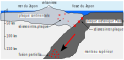
\includegraphics[scale=1]{../Figures_chap_intro/tectonik.pdf}
\caption[Schéma d'une zone de subduction]{Schéma de la zone de subduction de la fosse océanique du Japon. La subduction d'une plaque océanique donne naissance à des séismes, mais aussi à de nombreux phénomènes géophysiques comme le volcanisme à l'origine des reliefs de l'île du Japon (adapté de\,\cite{beig_friction_2006}).}
\label{fig:japon}
\end{figure}

\newpage

\minitoc
\newpage




\section{Les frottements solides}
\label{sec:frot}

\subsection{Que sont les frottements ?}

Les termes de \textit{frottement} ou de \textit{friction} désignent l'ensemble des interactions qui s'appliquent à deux systèmes mécaniques en contact et qui s'opposent à leur mouvement.
Le domaine de la physique qui étudie les frottements solides, la \textit{tribologie}, est définie comme la science de l'usure, des frottements et de la lubrification.
%Les phénomènes de frottement sont omniprésents tant dans notre quotidien que dans les applications technologiques de pointe ou les évènements géophysiques
Ces phénomènes sont omniprésents dans notre quotidien. Nous les retrouvons par exemple dans le simple fait de marcher, puisque c'est l'existence d'un frottement solide entre nos chaussures et le sol qui nous propulse en avant. Ceci est bien illustré par la grande difficulté avec laquelle
%\href{https://youtu.be/qQE-lMtGaN8}{\textcolor{black}{nous nous déplaçons sur la glace}},
nous nous déplaçons sur la glace,
surface à frottements faibles\,\cite{bowden_friction_1953}.


Cette section discute, par une approche historique, des mécanismes et modélisations du frottement solide. Ces mécanismes sont une première approche de la mécanique des failles, en particulier des séismes, qui peuvent être décrits comme la manifestation d'un mouvement de stick-slip, caractéristique des interfaces frictionnelles\,\cite{brace_stick-slip_1966}. 

\subsection{Origine microscopique des forces de frottement macroscopiques}

\begin{figure}[htb]
\centering
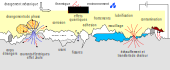
\includegraphics[scale=1]{../Figures_chap_intro/microscopic_complexity.pdf}
\caption[Complexité d'une interface réelle]{Visualisation schématique d'un contact frictionnel réel, et des interactions à l'œuvre à l'interface. L'aire de contact réelle entre les deux solides est nettement plus faible que l'aire de contact apparente.}
\label{fig:asperit}
\end{figure}




Lors d'un contact frictionnel entre deux objets, les frottements solides se manifestent à l'échelle macroscopique par l'apparition d'une force opposée à leur mouvement relatif. L'origine de cette force est à chercher à l'échelle microscopique. Une surface qui nous apparaît lisse au toucher est en réalité rugueuse, couverte d'aspérités dont la position et la taille sont aléatoires, à la manière d'un papier abrasif microscopique, allant selon les matériaux et traitements de surfaces du nanomètre au millimètre. Lors de la mise en contact de deux solides, ces aspérités s'entremêlent, répartissant la force pressante sur de multiples points de contacts, nommés \textit{microcontacts}. Ces points sont le siège d'un ensemble complexe d'interactions électrostatiques, chimiques et mécaniques, dans lesquelles interviennent les deux surfaces rugueuses des solides, mais également les impuretés et corps étrangers présents entres ceux-ci (Fig.\,\ref{fig:asperit}). La complexité de ces interactions rend irréaliste l'étude du comportement d'une interface rugueuse par le calcul exact de toutes les forces qui s'y exercent. L'étude de ces interfaces s'est donc historiquement faite au travers de lois empiriques macroscopiques telles que les lois d'Amontons-Coulomb (Sec.\,\ref{sec:coulomb}), puis par des lois justifiées par des modèles microscopiques des contacts à l'interface, comme le modèle de Bowden et Tabor, puis les modèles dits \textit{Rate-and-State} (Sec.\,\ref{sec:microfric}).

La prochaine section est dédiée aux premières tentatives de la modélisation de la friction solide par les lois d'Amontons-Coulomb.


\subsection{Description macroscopique -- Lois d'Amontons-Coulomb}
\label{sec:coulomb}


\begin{figure}[htb]
\centering
\includegraphics[width=.45\textwidth]{../Figures_chap_intro/vinci.png}
\caption[Croquis de Léonard de Vinci]{Croquis de Léonard de Vinci au sujet du frottement d'un objet sur une surface. Les dessins représentent des expériences d'étude de la friction par traction dans lesquelles différents objets sont tractés par une masse leur étant reliée par une cordelette et une poulie (adapté de\,\cite{hutchings_leonardo_2016}).}
\label{fig:vinci}
\end{figure}

Bien que les premiers écrits sur les frottements solides remontent à l'antiquité romaine, Thémistios écrivant notamment au quatrième siècle dans son \textit{De la Physique} «\,Il est plus facile d'entretenir le mouvement d'un corps se déplaçant que d'initier celui d'un corps au repos\,»\,\cite{themistius_aristotle_2008}, la première modélisation des frottements solides est due à Léonard de Vinci au XV\up{ème} siècle, dans son \textit{Codex Atlanticus} (Fig.\,\ref{fig:vinci})\,\cite{hutchings_leonardo_2016}. Ces travaux, redécouverts par Guillaume Amontons en 1699, et complétés par Leonhard Euler (1750) et Charles-Augustin de Coulomb (1785), ont abouti à la modélisation du problème à deux corps en contact frictionnel et à l'établissement de trois lois macroscopiques permettant de le résoudre.

\subsubsection{Définition du problème}

\begin{figure}[htb]
\centering
\includegraphics[scale=1]{../Figures_chap_intro/coulomb.pdf}
\caption[Référentiel utilisé pour les lois de Coulomb]{Définition du système étudié. Le référentiel choisi est celui du laboratoire muni d'un repère orthonormé direct $\left(\vec{e_x},\,\vec{e_y},\,\vec{e_z}\right)$. Le plan dans lequel le contact entre la masse et la surface s'effectue est le plan  $\left(\vec{e_x},\,\vec{e_z}\right)$, et $\vec{e_y}$ est pris orthogonal à ce plan, et orienté vers le haut (et de manière plus générale dans la direction opposée à la force pressante).
}
\label{fig:coulomb}
\end{figure}

Le système que nous considérons dans le cadre de la friction entre deux solides est une masse $m$ indéformable dont la surface macroscopiquement lisse d'aire $A$ est déposée sur un support horizontal immobile (Fig.\,\ref{fig:coulomb}). Sa vitesse est notée $\vec{v}$, et la direction de la vitesse $\vec{u_v} = \vec{v}/\norm{\vec{v}}$. Nous nommons \textit{force normale} $\vec{F_N}$, ou force pressante, la projection de la somme des forces appliquées à la masse sur le vecteur normal à l'interface, en excluant la réaction du support.

Les phénomènes de friction entrent en jeu lorsqu'une force tend à mettre en mouvement le solide, et a donc une composante tangentielle à l'interface. Ils se manifestent par l'apparition d'une force $\vec{F_f}$, qui s'applique dans le plan de l'interface, dans la direction contraire au sens de la mise en mouvement. Nous nommerons alors \textit{force cisaillante} $\vec{F_S}$ la projection de toutes les forces appliquées à la masse dans le plan de l'interface, à l'exception de cette force de réaction due aux frottements (Fig.\,\ref{fig:coulomb}).

Le problème étant ainsi défini, nous pouvons énoncer les trois lois d'Amontons-Coulomb décrivant la force de frottement $\vec{F_f}$ en fonction des forces normale $\vec{F_N}$ et cisaillante $\vec{F_S}$ appliquées à la masse $m$.


\subsubsection{Lois d'Amontons-Coulomb}

La modélisation du comportement d'une interface frictionnelle repose sur trois lois fondamentales, nommées d'après ceux qui les ont découvertes et rendues publiques, Guillaume Amontons (1699) et Charles-Augustin de Coulomb (1785).

\myparagraph{Lois du frottement statique -- \boldmath$\mu_s$}

La première loi d'Amontons affirme que pour mettre en mouvement la masse lorsqu'elle est immobile, il faut lui appliquer une force cisaillante telle que $F_S=\mu_sF_N$, où $\mu_s$ est une constante nommée \textit{coefficient de frottement statique}. Elle s'écrit

\begin{equation}
\text{tant que }{v}=0\qquad
\begin{aligned}\left\{
	\begin{split}
		\max F_f &= \mu_s F_N\\
		\vec{F_f} &= -\vec{F_S}\\
	\end{split}
	\right.
\end{aligned}
\end{equation}


La deuxième loi d'Amontons stipule que la force de frottement, notamment $\mu_s$, ne dépend pas de l'aire de contact apparente entre les deux solides.


\myparagraph{Loi du frottement dynamique -- \boldmath$\mu_d$}


La troisième loi de la friction, ou loi de Coulomb, précise qu'une fois que le solide est mis en mouvement relativement au support, la force de frottement qu'il subit est toujours opposée à la direction du mouvement et de norme constante, indépendante notamment de sa vitesse de glissement. Cette troisième loi nous permet de définir le \textit{coefficient de frottement dynamique} $\mu_d$ tel que

\begin{equation}
\vec{F_f} = - \mu_d F_N\,\vec{u_v}
\end{equation}


Une conséquence intéressante de cette loi est que la force de frottement est non-conservative, puisque son travail dépend du chemin suivi par l'objet sur lequel elle s'applique. Sur un chemin $\mathscr{C}$ de longueur $L_{\mathscr{C}}$,  à force normale constante, le travail $W_{\mathscr{C}}(\vec{F_f})$ vaut


\begin{equation}
W_{\mathscr{C}}(\vec{F_f})
= \int_{\mathscr{C}}\vec{F_f}\cdot\mathrm{d}\vec{u_v}
= -\mu_dF_N
\times \int_{\mathscr{C}}\vec{u_v}\cdot\mathrm{d}\vec{u_v} 
= -\mu_dF_NL_{\mathscr{C}}
\label{eq:dissip}
\end{equation}

Ce travail étant toujours négatif, la force de frottement dynamique fait toujours perdre au système de l'énergie. L'énergie perdue, dissipée en chaleur, est proportionnelle à la distance parcourue par l'objet.




\subsubsection{Variabilité des coefficients de frottement}

Émergeant des lois d'Amontons-Coulomb, $\mu_s$ et $\mu_d$ peuvent être considérés comme des grandeurs caractéristiques d'une interface entre deux matériaux donnés. Selon les conditions expérimentales (état de surface, lubrification, humidité ambiante, etc.) ces coefficients varient, mais à conditions expérimentales fixées il est possible de tabuler leurs valeurs (Fig.\ref{table:coef}). Cependant même en conditions expérimentales contrôlées, les coefficients varient d'un échantillon à un autre, et d'une expérience à l'autre, d'un facteur typiquement de l'ordre de 10\%, et leur utilisation nécessite un regard critique\,\cite{ben-david_static_2011, blau_significance_2001, czichos_multilaboratory_1987} (Fig.\,\ref{fig:disparite}). L'indépendance de $\mu_d$ de la vitesse de glissement notamment est une approximation dont les limites sont expérimentalement observées (Sec.\,\ref{sec:evolutionmacro}).


% Émergeant des lois d'Amontons-Coulomb, $\mu_s$ et $\mu_d$ sont souvent considérés comme des grandeurs caractéristiques d'une interface entre deux matériaux donnés. En réalité ils dépendent des conditions expérimentales dans lesquelles les deux matériaux sont frottés, en particulier de l'état de surface de ceux-ci, ou de la présence de corps étrangers. Ces variations donnent lieu à des tables de valeurs de coefficients de frottement entre différents matériaux et dans différentes conditions (Fig.\ref{table:coef}). Même en conditions contrôlées, ces coefficients sont très variables d'un échantillon à l'autre, et d'une expérience à l'autre, et leur utilisation nécessite un regard critique\,\cite{ben-david_static_2011, blau_significance_2001, czichos_multilaboratory_1987} (Fig.\,\ref{fig:disparite}). L'indépendance de $\mu_d$ de la vitesse de glissement notamment est une approximation dont les limites sont expérimentalement observées (Sec.\,\ref{sec:evolutionmacro}).

\begin{figure}[htb]
\centering
\begin{tabular}{ |p{4.5cm}||p{3cm}|p{3cm}|  }
 \hline
 \multicolumn{3}{|c|}{Coefficient de frottement statique} \\
 \hline
 \textbf{Matériau de la corde}& \textbf{Sèche} & \textbf{Humide} \\
 \hline
 Nylon         & 0.10 -- 0.12 &  0.12 -- 0.15\\
 Polyester     & 0.12 -- 0.15 &  0.15 -- 0.17\\
 Polypropylène & 0.08 -- 0.11 &  0.08 -- 0.11\\
 Aramide        & 0.12 -- 0.15 &  0.15 -- 0.17\\
 HMPE          & 0.08 -- 0.11 &  0.08 -- 0.11\\
 \hline
\end{tabular}
\caption[Exemple de table de coefficients de frottement statique]{Exemple de table de coefficients de frottement statique. Sont tabulés ici les coefficients de frottement entre une plaque d'acier lisse et des cordes de différents matériaux, sèches ou humides\,\cite{mckenna_properties_2004}.}
\label{table:coef}
\end{figure}

\begin{figure}[htb]
\centering
\includegraphics[width=.6\textwidth]{../Figures_chap_intro/multilab.png}
\caption[Variabilité du coefficient de frottement]{Coefficients de frottement dynamique mesurés par différentes équipes de recherche sur des échantillons identiques en acier. Chaque point représente une expérience, et chaque colonne de points l'ensemble des résultats d'un laboratoire (extrait de\,\cite{ czichos_multilaboratory_1987}). Moyenne : $0.6$, écart type : $0.109$.}
\label{fig:disparite}
\end{figure}




\subsubsection{Émergence du phénomène de stick-slip}
\label{sec:ss1}

\begin{figure}[htb]
\centering

\includegraphics[scale=1]{../Figures_chap_intro/stickslip.pdf}
\caption[Mouvement de stick-slip sur un tapis roulant]{\textbf{a.} Système mécanique pouvant aboutir à un mouvement de stick-slip. \textbf{b.} Évolution temporelle typique de la longueur du ressort dans ce système. Les axes sont en unités arbitraires, de tels mouvements pouvant se produire à des échelles très variées.}
\label{fig:shemastickslip}
\end{figure}

Le phénomène de stick-slip, ou collé-glissé, est un mouvement saccadé entre deux solides liés par une interface frictionnelle, qui émerge de la différence entre $\mu_s$ et $\mu_d$.
Pour le mettre en évidence, considérons un système modèle composé d'une masse $m$, reliée à un support immobile par un ressort idéal de raideur $k$, et placée sur un tapis roulant évoluant à vitesse constante $v$ (Fig.\,\ref{fig:shemastickslip}). Alors si $\mu_d<\mu_s$, le mouvement se décompose en deux phases qui alternent :

\begin{itemize}
\bitem \textit{Stick} : les deux solides sont solidaires, leur mouvement relatif est nul, les lois d'Amontons décrivent les interactions frictionnelles entre les deux par le biais du coefficient de frottement statique $\mu_s$. Durant cette phase, l'interface se charge en cisaillement par les déformations du ressort.
\bitem \textit{Slip} : les deux solides se mettent en mouvement relatif, ils glissent, la troisième loi de Coulomb décrit le mouvement par le coefficient $\mu_d$.
\end{itemize}


Les lois d'Amontons Coulomb permettent d'aboutir à la description d'un mouvement périodique, de période $T_{ss}$,  et d'amplitude $A_{ss}$, qui en posant $\omega_0 = \sqrt{{k}/{m}}$ s'écrivent


\begin{align}[left=\empheqlbrace]
	\begin{split}
		T_{ss} &= 2\frac{(\mu_s-\mu_d) \,g}{\omega_0^2\,v} + \dfrac{\pi}{\omega_0}\\
		A_{ss} &= \frac{(\mu_s-\mu_d)\,g}{\omega_0 ^2}
	\end{split}
\label{eq:freqss}
\end{align}



Les lois d'Amontons-Coulomb permettent de décrire synthétiquement de nombreux systèmes frictionnels, mais sont limitées en raison des variations des coefficients de frottement en fonction du temps et de la vitesse, et de l'hétérogénéité des interfaces réelles. Elles ont été énoncées à leur origine sans justification microscopique, et relèvent d'une description empirique d'interfaces macroscopiques. Un modèle microscopique historiquement utilisé pour les décrire est détaillé dans la section suivante.



\subsection{Modèles microscopiques de la friction}

\label{sec:microfric}



La description par des modèles macroscopiques du frottement entre deux solides s'appuie historiquement sur des observations empiriques. Les modèles microscopiques justifiant de la validité des trois lois d'Amontons-Coulomb sont récents (\textsc{xx}\up{ème} siècle), avec notamment le modèle de Bowden et Tabor\,\cite{bowden_friction_1950}, publié en 1950. Ces modèles reposent sur la prise en compte de la réalité microscopique des contacts entre les deux solides.


\subsubsection{Description de l'aire de contact réelle}

\begin{figure}[h]
\centering	
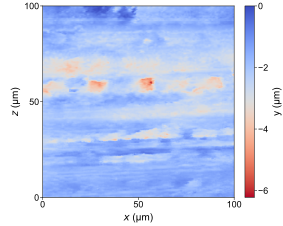
\includegraphics[scale=1]{../Figures_chap_intro/profiloplot_zoom.pdf}
\caption[Profil microscopique d'un bloc de PMMA]{Profil d'altitude d'une portion de bloc de plastique poli  à l'aide de papier abrasif fin (P1200). L'altitude de référence est la surface macroscopique du bloc. Les aspérités, dont la hauteur est de l'ordre de quelques micromètres, semblent aléatoirement distribuées. Cet échantillon présente des traces d'usure, sous la forme de rainures le long de l'axe $x$.}
\label{fig:asperit2}
\end{figure}


Lorsque deux solides sont en contact, l'aire de contact réelle entre les microaspérités à l'interface est bien plus faible que l'aire apparente macroscopique de contact $A$ (Fig.\,\ref{fig:asperit2}). Lors de la mise en contact de deux solides, seules les plus hautes aspérités de chaque surface se rencontrent. L'aire réelle de contact est nommée $A_r$ et peut être décrite comme la somme des aires de chaque aspérité en contact. Cette aire est par exemple mesurable dans les solides transparents par des méthodes optiques reposant sur la réflexion interne totale de la lumière\,\cite{dieterich_direct_1994}.
Afin de modéliser le contact entre les deux solides, un modèle du comportement des microcontacts soumis à une pression et de leur distribution est nécessaire.

La mécanique des contacts est un domaine de recherche riche et actif, et nous n'en proposons dans ce chapitre qu'un aperçu, au travers de deux modèles historiques de contacts uniques. Il  existe cependant d'autres méthodes pour aborder ce type de problèmes, plus récentes et plus précises\,\cite{greenwood_contact_1966, derjaguin_effect_1975,  johnson_surface_1971, maugis_adhesion_1992, persson_theory_2001, vakis_modeling_2018}, que nous n'aborderons pas ici.




Dans cette section, de façon à distinguer les forces macroscopiques $F_N$ et $F_S$ des forces à l'échelle des microcontacts, nous nommerons en minuscule $f_n$ et $f_s$ les forces appliquées sur un microcontact de surface $A_\mu$, de telle sorte qu'une contrainte $\sigma$ subie par ce microcontact s'écrive $\sigma=f/A_\mu$.


\subsubsection{Modèles d'aspérités}




Nous présentons deux modèles d'aspérités sans adhésion, selon que la pression de contact est faible, et les déformations élastiques, ou que la pression est forte, et les déformations plastiques.

\myparagraph{Aspérité élastique}

Pour une aspérité individuelle élastique, de module d'Young $E$ et de coefficient de Poisson $\nu$, nous noterons $E^*={E}/(1-\nu^2)$. Dans le cadre du contact de Hertz\,\cite{hertz_ueber_1882}, si cette aspérité dispose d'un rayon de courbure $\rho_r$ et est pressée contre une surface dure sous une force normale $f_n$, alors son aire de contact avec cette surface est

\begin{equation}
A_\mu = \pi\left(\frac{3}{4}\times\frac{1}{E^*}\times\rho_r\times f_n\right)^{2/3}\propto f_n^{2/3}
\end{equation}



Ainsi l'aire de contact augmente proportionnellement à $f_n^{2/3}$, tandis que la pression subie par le contact, $f_n/A_\mu$, augmente proportionnellement à $f_n^{1/3}$.


\myparagraph{Aspérité plastique}

\begin{figure}[htb]
\centering
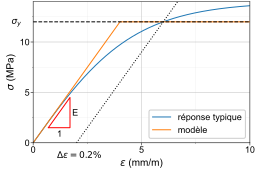
\includegraphics[scale=1]{../Figures_chap_intro/yield.pdf}
\caption[Limite de plasticité d'un matériau]{Réponse contrainte-déformation d'un matériau plastique typique, avec $E=\SI{3}{\giga\pascal}$ et $\sigma_Y=\SI{12}{\mega\pascal}$. En bleu, exemple de réponse typique du matériau. Dans les régimes que nous considérons, la contrainte est une fonction croissante de la déformation. Nous la modélisons par la courbe orange. Ce modèle comporte d'abord une réponse purement élastique, telle que si $\varepsilon<\sigma_Y/E$ alors $\sigma=E\varepsilon$, puis une réponse purement plastique, telle que si $\varepsilon\geq\sigma_Y/E$, alors $\sigma = \sigma_Y$. La définition communément acceptée de $\sigma_Y$, représentée par les lignes pointillées, est la valeur de contrainte telle qu'une fois le matériau de nouveau déchargé, sa déformation plastique soit de 0.2\%\,\cite{avallone_marks_2006}.}
\label{fig:yield}
\end{figure}




Si les contraintes subies par les microcontacts sont grandes les déformations sont plastiques, et $\sigma$ atteint un maximum. La contrainte limite d'élasticité $\sigma_Y$ (\textit{yield stress}, homogène à une pression) est définie comme la contrainte à partir de laquelle les déformations de l'aspérité deviennent plastiques (Fig.\,\ref{fig:yield}). La valeur de $\sigma_Y$ est une caractéristique du matériau. Les valeurs typiques de $\sigma_Y$ sont de l'ordre de quelques $10^7\,\text{Pa}$ pour la plupart des matériaux polymères rigides\,\cite{avallone_marks_2006}. Cela correspond environ à dix fois la contrainte normale que nous appliquons sur la surface \textit{apparente} de nos échantillons expérimentaux (Sec.\,\ref{sec:echantillons}).

Si une force normale $f_n$ est appliquée sur un microcontact plastique de surface de contact $A_{\mu}$, celle-ci ne pouvant supporter qu'une contrainte normale $\sigma_n=\sigma_Y$, alors

\begin{equation}
A_\mu = \frac{f_n}{\sigma_Y}
\label{eq:microcontact}
\end{equation}

Ainsi, $A_\mu$ augmente linéairement avec $f_n$.


\myparagraph{Cisaillement d'une aspérité}

Qu'il soit élastique ou plastique, un microcontact résiste au glissement tant qu'il n'est pas brisé ou affaibli. Sa résistance au cisaillement $\sigma_r$ correspond à la contrainte cisaillante maximale qu'il peut supporter sans glisser. La force cisaillante $f_s$ maximum que le microcontact peut retenir est donc

\begin{equation}
\max f_s = A_\mu\times \sigma_r
\end{equation}

Ainsi la force cisaillante maximale que peut supporter un microcontact avant de glisser augmente linéairement avec $A_\mu$.

\pagebreak

En conclusion, ces deux modèles montrent que la surface d'un microcontact augmente avec la force normale qu'il porte. Elle est proportionnelle à la force normale dans le cas d'un microcontact plastique, tandis que pour un microcontact élastique elle est proportionnelle à $f_n^{2/3}$. La force cisaillante que peut retenir un microcontact est pour sa part proportionnelle à cette surface. Ces modèles de microcontacts peuvent maintenant être appliqués à l'échelle d'une interface toute entière.




\subsubsection[Modèle d'interface -- lois d'Amontons-Coulomb]{Modèle d'interface -- justification des lois d'Amontons-Coulomb}
\label{sec:amontonsmicro}

Nous restreignons cette présentation au cas d'une interface dont les contacts ont un comportement plastique car les matériaux que nous étudions dans les conditions choisies sont correctement décrits par ce modèle\,\cite{rubinstein_crack-like_2006}. Cependant les résultats présentés resteraient valides pour une interface partiellement ou entièrement élastique avec une distribution gaussienne des hauteurs des aspérités\,\cite{singer_contact_1992}.

\myparagraph{Frottement statique}

Dans le cas d'une interface plastique, le modèle de Bowden et Tabor\,\cite{bowden_friction_1950} décrit la surface comme un ensemble de microcontacts de surfaces $\{A_{\mu,i}\}_i$. La force normale portée par l'interface peut alors s'écrire comme la somme des forces normales portées par l'ensemble des microcontacts, $F_N = \sum_if_{n,i}$. En appliquant l'Équation\:\ref{eq:microcontact} à chacun de ces microcontacts nous obtenons

\begin{equation}
A_r = \sum_i A_{\mu,i} = \sum_i\frac{f_{n,i}}{\sigma_Y} = \frac{F_N}{\sigma_Y}
\label{eq:wamu}
\end{equation}

Ainsi l'aire de contact réelle $A_r$ de l'interface est proportionnelle à la force normale $F_N$ qui lui est appliquée. En appliquant un raisonnement similaire sur la force cisaillante, répartie sur tous les microcontacts, nous obtenons $\max F_S = \sum_i \max f_{s,i} = \sum_i  \sigma_rA_{\mu,i} = \sigma_r A_r$. Ainsi le coefficient de frottement statique se définit comme

\begin{equation}
\max F_S = \mu_sF_N\qquad\text{avec} \qquad \mu_s = \dfrac{\sigma_r}{\sigma_Y}
\label{eq:maxfs1}
\end{equation}



Au travers cette modélisation microscopique nous retrouvons les deux lois d'Amontons, ainsi qu'une définition du coefficient de frottement statique. Cette définition reste sujette à discussion, puisqu'elle repose sur l'utilisation de $\sigma_Y$ et $\sigma_r$. La contrainte limite d'élasticité $\sigma_Y$ est une caractéristique du matériau, et la considérer constante est une bonne approximation. La résistance au cisaillement $\sigma_r$ pour sa part n'est pas une grandeur caractéristique. Elle dépend de la géométrie des contacts et de chaque aspérité considérée, et n'est pas à priori connue.


\myparagraph{Frottement dynamique}


Lorsque l'interface est en glissement quasi-statique, les microcontacts se cassent et se reforment de manière répétée. La formation d'un point de contact s'accompagne de l'accumulation rapide de contraintes cisaillantes sur ce point, puis à une nouvelle mise en glissement. Les deux aspérités poursuivent leur glissement jusqu'à rencontrer une nouvelle aspérité avec laquelle répéter ce cycle. Tandis que le solide glisse de manière quasi-statique, les microcontacts subissent des mouvements rapides et irréguliers\,\cite{persson_sliding_1998,beig_friction_2006}. En reprenant la description du contact unique cisaillé proposée plus haut (Éq.\,\ref{eq:wamu} et\,\ref{eq:maxfs1}), chaque rupture de microcontact s'effectue à une force cisaillante $f_s$ telle que

\begin{equation}
f_s=A_\mu\times\sigma_r= \dfrac{\sigma_r}{\sigma_Y}f_n
\end{equation}

Ainsi, peu importe la vitesse à laquelle le glissement est effectué, si nous considérons comme isotrope la répartition des microcontacts, la force cisaillante macroscopique $F_S$ est de valeur constante

\begin{equation}
F_S = \mu_dF_N\qquad\text{avec} \qquad \mu_d = \mu_s = \dfrac{\sigma_r}{\sigma_Y}
\label{eq:maxfs}
\end{equation}


Les limitations de ce modèle sont ainsi mises en exergue, puisqu'il ne parvient pas à prédire de différence entre $\mu_s$ et $\mu_d$, ni l'évolution de ces deux coefficients en fonction du temps et de la vitesse de glissement observée expérimentalement pour des interfaces solide-solide réelles.



\subsection[Modélisation de l'évolution de $\mu$]{Modélisation de l'évolution des coefficients de frottement}
\label{sec:evolutionmacro}

Les coefficients de frottement ne sont pas des caractéristiques d'une interface, comme décrit précédemment. Le coefficient de frottement statique tend à augmenter avec l'âge de l'interface, tandis que le coefficient de frottement dynamique, à l'inverse de ce que stipule la troisième loi de Coulomb, dépend de la vitesse de glissement. Cette section décrit ces observations et un modèle empirique permettant d'en rendre compte.

\subsubsection{Vieillissement d'une interface au repos}
\label{sec:aging}

\begin{figure}[htb]
\centering
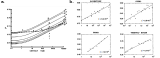
\includegraphics[scale=1]{../Figures_chap_intro/aging.pdf}
\caption[Vieillissement d'une interface bloquée]{\textbf{a.} Évolution du coefficient de frottement statique $\mu$ en fonction du temps de contact normalisé ($\tau=\theta/\theta_0$) pour différentes roches (extrait de\,\cite{dieterich_modeling_1979}). Les échantillons étudiés sont des granodiorites californiennes poncées avec des papiers abrasifs P60 à P600. Pour tous les échantillons présentés, le coefficient augmente proportionnellement au logarithme de l'âge de l'interface. \textbf{b.} Évolution du coefficient de frottement statique $\mu_s$ en fonction du temps de contact $\tau$ dans divers matériaux (extrait de\,\cite{baumberger_contact_1997}). La ligne est un ajustement des points de la forme $\mu(\tau)=\mu_0+\text{b}\ln\tau$.}
\label{fig:aging}
\end{figure}



Le coefficient de frottement statique augmente logarithmiquement avec le temps de contact entre les deux solides (Fig.\,\ref{fig:aging}), dans tous les matériaux, y compris les roches et les matières plastiques\,\cite{dieterich_modeling_1979,baumberger_contact_1997} comme le polyméthacrylate de méthyle (PMMA) que nous utilisons dans nos expériences (Sec.\,\ref{sec:materials}). Ce vieillissement (\textit{aging}) s'explique par une augmentation logarithmique de la surface réelle de contact $A_r$. Le mécanisme sous-jacent est que les microcontacts, de part leur échelle microscopique, s’étalent avec le temps sous l'effet de l'agitation thermique. Telles des particules dans un potentiel comportant des minima locaux, lorsque ces aspérités sont soumises à des fluctuations thermiques, elles sautent de minimum en minimum, augmentant progressivement l'aire de contact réelle entre les deux surfaces. Ce phénomène est nommé \textit{fluage} (\textit{indentation creep})\,\cite{cocks_indentation_1991,dieterich_direct_1994,baumberger_solid_2006}.



\subsubsection[Influence de la vitesse sur $\mu$]{Influence de la vitesse sur le coefficient de frottement}

\begin{figure}[htb]
\centering
\includegraphics[scale=1]{../Figures_chap_intro/speed_mu.pdf}
\caption[Évolution de $\mu$ lors d'un saut de vitesse]{Évolution du coefficient de frottement dynamique en fonction de la vitesse (adapté de\,\cite{dieterich_modeling_1979}). Les échantillons étudiés sont des granodiorites d'une carrière californienne poncées avec du papier abrasif. La vitesse de déplacement varie au cours de l'expérience.}
\label{fig:speed_mu}
\end{figure}





Lorsqu'un solide est en glissement sur une surface, son coefficient de frottement évolue en fonction de la vitesse de glissement $V$ (Fig.\,\ref{fig:speed_mu}). En régime de glissement stable, $\mu$ est proportionnel au logarithme de  $V$\,\cite{ruina_slip_1983,stesky_mechanisms_1978,blanpied_frictional_1987,dieterich_direct_1994}. Lors d'un saut de vitesse positif, à temps court, $\mu$ augmente, puis relaxe à temps long vers une nouvelle valeur stable. Ce comportement provient de la concurrence de deux effets. L'augmentation initiale de $\mu$ est l'effet de la résistance intrinsèque des contacts\,\cite{dieterich_direct_1994}. La diminution qui s'en suit relève d'un mécanisme de fluage similaire à celui à l'œuvre dans le vieillissement d'une interface au repos.
L'interface est le siège d'une compétition entre le renouvellement des contacts par son glissement et le vieillissement des contacts sous une charge normale.
%Plus la vitesse est élevée, moins les contacts nouvellement formés ont le temps de vieillir avant d'être à nouveau brisés.


Ces deux dépendances logarithmiques de $\mu$ en temps et en vitesse peuvent être décrites par des loi empiriques telles que celle proposée par Dieterich et Ruina en 1979 et 1983, que nous présentons ci-dessous.

\subsubsection{Modèle de Dieterich et Ruina -- Rate-and-State}
\label{sec:rateandstate}


\begin{figure}[h!]
\centering
\includegraphics[scale=1]{../Figures_chap_intro/velocity_s_w.pdf}
\caption[Comportement du modèle Rate-and-State]{Schéma du comportement d'un système frictionnel suivant une loi Rate-and-State, en fonction des paramètres $A$ et $B$ du modèle (adapté de\,\cite{zhang_frictional_2022}). La courbe rouge (resp. bleue) présente une friction renforcée (resp. affaiblie) par la vitesse.}
\label{fig:velocity_s_w}
\end{figure}

\newpage

Le modèle de Dieterich et Ruina\,\cite{dieterich_modeling_1979,ruina_slip_1983} est un modèle \textit{Rate-and-State} (\textit{taux-état}, rarement traduit dans la littérature), reliant le coefficient de frottement $\mu$ à la vitesse de glissement $V$ et à une fonction d'état $\theta$, selon l'équation 

\begin{equation}
\mu = \mu_0+A\ln\left(1+\frac{V}{V_0}\right)+B\ln\left(1+\frac{\theta}{\theta_0}\right)
\end{equation}


La loi décrite ici étant empirique, son interprétation physique est sujette à des réserves\,\cite{dieterich_direct_1994}. Il est cependant possible d'en trouver des justifications microscopiques\,\cite{baumberger_physical_1999, nakatani_conceptual_2001,chen_microphysically_2017}. Ainsi $\theta$ est généralement interprété comme l'âge des microcontacts formés entre les deux solides. Les constantes $\theta_0$, $\mu_0$ et $V_0$ sont déterminées expérimentalement.

Cette équation doit être couplée avec une équation d'état modèle pour l'évolution de $\theta$. L'équation proposée par Dieterich considère que l'âge des contacts évolue selon l'équation

\begin{equation}
\diff{\theta}{t} = 1-\frac{\theta V}{D_c}
\end{equation}

La constante $D_c$, homogène à une longueur, correspond à la distance de glissement caractéristique nécessaire pour renouveler entièrement une population de contacts. Ce modèle permet d'exprimer à vitesse nulle le coefficient de frottement statique et de rendre compte de son augmentation logarithmique avec le temps.

\begin{equation}
\mu_s=\mu_0+B\ln(1+\theta/\theta_0)
\end{equation}

Lorsque le glissement se fait en régime stationnaire, $V$ est constante et $\theta = D_c/V$. Nous considérons les cas où $V/V_0\gg1$ et $D_c/V\theta_0\gg1$, hypothèses généralement valides pour les systèmes que nous étudions. Le cas général ainsi que les limites inverses de ces hypothèses sont traités dans la littérature\,\cite{bar-sinai_slow_2012, barsinai_velocitystrengthening_2014,bar-sinai_velocity-strengthening_2015}. Nous obtenons alors


\begin{equation}
\mu = \text{const.}+(A-B)\ln(V)
\end{equation}


Ce modèle met en évidence deux constantes $A$ et $B$, représentant respectivement la résistance au cisaillement des contacts et celle du vieillissement statique. L'effet de $A$, nommé \textit{effet direct}, est visible à temps court et va toujours dans le sens de la résistance au changement de vitesse. L'effet de $B$, ou \textit{effet indirect}, est visible à temps longs, lorsque le glissement est supérieur à $D_c$ (Fig.\,\ref{fig:velocity_s_w}). Lorsque le vieillissement est dominant, $B>A$, le frottement est d'autant plus faible que la vitesse est grande, il est dit affaibli par la vitesse (\textit{velocity weakening}). Dans le cas inverse, $A>B$, le frottement est renforcé par la vitesse (\textit{velocity strengthening}).

Ce modèle, bien que justifié par des considérations microscopiques, reste empirique. Aussi d'autres lois d'évolution de $\theta$ existent, représentant plus fidèlement le comportement de l'interface lorsqu'elle est soumise à des variations rapides de vitesse. Toutes cependant permettent de rendre compte d'un écart entre $\mu_s$ et $\mu_d$, et de l'apparition de deux régimes de déplacement, le glissement stable et le stick-slip\,\cite{ruina_slip_1983,nagata_revised_2012,aharonov_physicsbased_2018}.


\subsubsection{Instabilité de stick-slip}


\begin{figure}[htb]
\centering

\includegraphics[scale=1]{../Figures_chap_intro/stability.pdf}
\caption[Diagramme de stabilité d'un mouvement de stick-slip]{\textbf{a.} Réponse d'un système masse-ressort posé sur un tapis roulant à vitesse constante. Lorsque la force normale décroît, le comportement de la masse effectue une transition entre un régime de stick-slip et un glissement permanent à vitesse variable, puis un glissement stable (adapté de\,\cite{baumberger_physical_1999}). \textbf{b.} Diagramme de stabilité schématique d'une interface affaiblie par la vitesse (adapté de \,\cite{scholz_earthquakes_1998}). Ce diagramme montre le saut de vitesse nécessaire afin de déstabiliser une interface en glissement stable, en fonction de la contrainte normale qui lui est appliquée. Le régime instable évolue en stick-slip quel que soit la perturbation de vitesse, tandis que le régime de stabilité conditionnelle n'évolue en stick-slip que si le saut de vitesse est suffisant.}
\label{fig:ss2}
\end{figure}


Dans le cas d'une interface à frottement renforcé par la vitesse, un mouvement de glissement est intrinsèquement stable. Une fluctuation de vitesse se traduit par un changement de vitesse de glissement stable. Une interface à frottement affaibli par la vitesse en revanche peut exhiber un comportement instable de stick-slip, comme conséquence de l'existence d'un coefficient de frottement dynamique inférieur au coefficient de frottement statique (Sec.\,\ref{sec:ss1}, Fig.\,\ref{fig:ss2}a). Ce comportement instable en vitesse est bien décrit par une bifurcation de Hopf\,\cite{rice_stability_1983,gu_slip_1984,heslot_creep_1994}. Si l'on considère un écart de vitesse $\Delta V$ appliqué à une interface en glissement stable, et $\sigma$ la pression normale appliquée sur l'aire de contact apparente $A$, il est possible de définir une valeur critique $\sigma_c$ de cette pression à laquelle le comportement du système passe d'un régime toujours instable à un régime conditionnellement stable (Fig\,\ref{fig:ss2}b).


Cette analyse de stabilité met en avant l'existence d'interfaces toujours en glissement stable car renforcées par la vitesse, et d'interfaces toujours instables car affaiblies par la vitesse et dans la zone instable du diagramme de bifurcation. Le modèle prédit également l'existence d'interfaces affaiblies par la vitesse, conditionnellement stables, nécessitant une fluctuation de vitesse pour entrer dans un régime de stick-slip. Cette fluctuation peut consister en la rupture partielle d'une interface, la portion instable de celle-ci entraînant une déstabilisation de sa portion conditionnellement stable. La détermination du caractère renforcé ou affaibli par la vitesse des portions de failles est à ce titre un enjeu majeur de l'étude des failles.




Le modèle Rate-and-State, couplé à une équation d'état, permet une bonne description de la dynamique d'une interface frictionnelle. Sa principale limitation réside dans son aspect empirique, nécessitant des ajustements pour déterminer les constantes $A$ et $B$ pour chaque système étudié. Dans un système de failles réelles, la connaissance des phénomènes à l'origine de leurs variations est nécessaire à l'étude et la prévision de la stabilité du mouvement. De plus les modèles présentés ne décrivent que le mouvement moyen de l'interface, celui du centre de masse du système, et ignorent son extension spatiale.

Cette dernière problématique soulève la question du mécanisme par lequel le mouvement s'initie. En effet cette initiation n'étant pas instantanée, elle doit s'accompagner d'un phénomène propagatif. Ce phénomène est la propagation d'une rupture interfaciale affaiblissant de proche en proche les microcontacts et permettant la mise en glissement de l'interface.



\newpage

\section{Mécanique de la fracture linéaire élastique}
\label{sec:LEFM}

Nous avons présenté dans la section précédente qu'une interface frictionnelle entre deux solides possède une structure complexe, étudiée au travers de modèles empiriques macroscopiques, justifiés par des considérations microscopiques. Ces modèles comme celui de Bowden et Tabor ou de Dieterich et Ruina font état de la réalité des contacts microscopiques à l'interface, mettant notamment en évidence la différence entre l' entre l'aire de contact réelle $A_r$ et l'aire de contact macroscopique $A$ aire de contact réelle $A_r$ et l'aire de contact macroscopique $A$ entre les deux solides. Ils ne fournissent cependant qu'un modèle pour le déplacement moyen des blocs à l'interface. 
%sur l'approximation que les solides en contact se déplacent %d'un bloc, sans déformations internes, comme infiniment rigides.
L'élasticité responsable de leur mouvement de stick-slip est alors extérieure au système, modélisable par un ressort effectif relié à une masse indéformable en frottement sur une surface fixe.
Dans la réalité pourtant l'élasticité provient des blocs en frottement eux-mêmes. Ils sont élastiques et se déforment, y compris à proximité de l'interface. Le changement brutal de vitesse lors d'une phase de slip n'est en réalité pas instantané. Tous les microcontacts n'entrent pas en glissement simultanément, mais s'affaiblissent de proche en proche au cours d'un phénomène propagatif, un \textit{crack} ou \textit{fracture}, ou encore \textit{rupture}.

La propagation de cette fracture s'accompagne de la libération dans le matériau d'ondes de compression et de cisaillement se propageant jusqu'en surface, et qui dans le cas des failles sismiques donnent naissance à un séisme. Cette rupture engendre une chute de contrainte cisaillante locale, et se déplace à des vitesses pouvant atteindre la vitesse du son dans le milieu. Elle correspond à une fracture en mode de cisaillement, décrite par la mécanique de la fracture linéaire élastique (LEFM, pour \textit{Linear Elastic Fracture Mechanics})\,\cite{svetlizky_brittle_2019}.


Dans cette section, nous présentons les principes de la propagation de fractures dans les matériaux et leur application à l'étude des frottements solides. La première partie décrit les bases de la théorie de l'élasticité que nous allons utiliser par la suite, la deuxième les fondements de la fracture statique puis dynamique, dont la théorie de Griffith, et la troisième l'application de la mécanique de la fracture linéaire élastique à la propagation de ruptures le long des interfaces frictionnelles.





\subsection{Mécanique du solide élastique}
\label{sec:hook}
La mécanique du solide élastique est le domaine de la physique qui décrit le comportement d'un objet solide ayant une réponse élastique linéaire lorsqu'il est soumis à des contraintes extérieures. Nous rappelons brièvement dans cette section la loi de Hooke régissant la réponse d'un solide élastique à une contrainte extérieure.

%\subsubsection{Loi de Hooke pour un ressort}


\begin{figure}[htb]
\centering
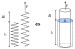
\includegraphics[scale=1]{../Figures_chap_intro/hooke.pdf}
\caption[Loi de Hooke pour un ressort]{Déformations d'un solide induites par une force extérieure. Tout solide élastique se comporte comme un ressort dont la raideur dépend de son module d'Young $E$ et de sa géométrie.}
\end{figure}


\newpage
%
%Lorsqu'un ressort idéal de longueur $l$ est soumis à une force de traction ou de compression, celui-ci se déforme, et produit une force $\vec{F}$ dans la direction opposée à la déformation en retour. Cette force est proportionnelle à l'étirement du ressort $\Delta l$, selon un coefficient de raideur $k$ de telle sorte que
%
%\begin{equation}
%F=-k\Delta l
%\end{equation}
%
%Le modèle du ressort décrit une pièce mécanique idéalisée, que l'on ne déformerait que selon un seul axe, et qui n'aurait qu'une seule dimension. Cette pièce se comporte alors comme un ressort, dont la longueur et la raideur sont déterminées par les propriétés du matériau qui la compose et sa géométrie. La loi de Hooke est une généralisation de la loi des ressors pour un solide.
%

\subsubsection{Loi de Hooke uniaxiale pour un solide élastique}

\myparagraph{Module d'Young}

%La géométrie d'une pièce mécanique est un facteur déterminant de sa réponse aux contraintes extérieures.
Lorsqu'une pièce mécanique est soumise à une force extérieure, l'étirement total qu'elle subit dépend de sa géométrie. À force égale, une barre deux fois plus longue s'allonge deux fois plus, tandis que la même force appliquée sur une surface deux fois plus grande l'allonge deux fois moins. Afin d'éliminer ces considérations, nous utilisons la contrainte $\sigma=F/A$ définie comme le rapport de la force $F$ appliquée sur la surface $A$, et l'allongement relatif, ou déformation, $\varepsilon=\Delta l/l_0$ défini comme le rapport entre l'allongement de la pièce $\Delta l$ et sa longueur à vide $l_0$. La \textit{loi de Hooke}\,\cite{hooke_potentia_1674} stipule alors qu'il existe un coefficient $E$ nommé \textit{module d'Young} tel que

\begin{equation}
\sigma=E\varepsilon
\end{equation}

Cette pièce se comporte alors comme un ressort, dont la raideur est déterminée par les propriétés du matériau qui la compose, sa longueur et sa géométrie. La loi de Hooke est une généralisation de la loi des ressorts pour un solide. Le module d'Young s'exprime en pascals. Pour le PMMA, matériau que nous utilisons dans cette étude, $E_{PMMA}\sim\SI{3}{\giga\pascal}$.
%et sa valeur varie typiquement du mégapascal pour les matériaux tels que le caoutchouc à plusieurs centaines de gigapascals pour les métaux\,\cite{feynman_feynman_1963}.

\myparagraph{Coefficient de Poisson}

La pièce raccourcie ou allongée sous l'effet de la contrainte voit également sa largeur changer. Lorsqu'un matériau est soumis à une contrainte $\sigma_\parallel$ selon un axe, il subit une déformation $\varepsilon_{\parallel} =\sigma_{\parallel} /E$ selon cet axe, mais également une déformation $\varepsilon_\perp$ dans le plan orthogonal à cet axe. Le \textit{coefficient de Poisson} est alors défini comme


\begin{equation}
\nu = -\frac{\varepsilon_\perp}{\varepsilon_{\parallel} }
\end{equation}


Le coefficient de Poisson est sans unité. Il prend des valeurs entre 0 et 0.5 et varie typiquement de 0.1 à 0.4 dans la plupart des matériaux courants\,\cite{feynman_feynman_1963}.

\subsubsection{Loi de Hooke généralisée}

Si l'on s'intéresse maintenant à une contrainte non unidirectionnelle, les contributions des contraintes s'additionnent. Il nous faut considérer le cas d'un petit cube de matière infinitésimal soumis à des contraintes, exprimées sous la forme d'un tenseur $[\sigma] = [\sigma_{i,j}]_{i,j\in\{1,2,3\}}$, où 1, 2 et 3 représentent les trois directions d'un repère orthonormé. Il en va de même pour $[\varepsilon]$. Sous l'hypothèse que le matériau est homogène et isotrope, toujours vérifiée par la suite, la loi de Hooke se généralise\,\cite{feynman_feynman_1963} sous la forme

\begin{equation}
[\sigma] = \frac{E}{1+\nu }\left( [\varepsilon] +\frac{\nu }{1-2\nu }\operatorname{Tr}\left( [\varepsilon] \right) \mathbf I_3 \right) 
\end{equation}

Soit encore en convention de sommation d'Einstein

\begin{equation}
\sigma_{ij} = \frac{E}{1+\nu } \left( \varepsilon_{ij}+\frac{\nu }{1-2\nu }\varepsilon_{kk} \delta _{ij}\right)
\end{equation}


Ainsi nous disposons d'une relation close permettant de lier les déformations aux contraintes subies par un matériau. Couplées à des conditions aux limites et des informations sur la géométrie des pièces considérées, cette équation nous permet de résoudre entièrement le problème de la répartition des contraintes. Dans notre étude nous utilisons des pièces dont la forme est celle de plaques minces, qui nous permettent de considérer un système 2D à trois degrés de liberté.


\subsubsection{Cas des plaques}

Une \textit{plaque} est une pièce dont la forme est celle d'un parallélépipède dont une des dimensions, notée $z$, est beaucoup plus faible que les autres. Sous la condition que la pièce est une plaque mince, nous pouvons effectuer l'hypothèse dite de \textit{planéité des contraintes} (\textit{plane stress}), qui considère que les contraintes appliquées selon l'axe $z$ sont toutes nulles, c'est à dire que $\sigma_{xz}=\sigma_{yz}=\sigma_{zz}=0$. Sous cette hypothèse la loi de Hooke se réécrit\,\cite{freund_dynamic_1990}


\begin{equation}
\begin{pmatrix}
\sigma_{xx} \\
\sigma_{yy} \\
\sigma_{xy}
\end{pmatrix}
=
\dfrac{E}{1-\nu^2}\times\begin{pmatrix}
1 & \nu & 0 \\
\nu & 1 & 0 \\
0 & 0 & \frac{1-\nu}{2} 
\end{pmatrix}
\cdot
\begin{pmatrix}
\varepsilon_{xx} \\
\varepsilon_{yy} \\
\varepsilon_{xy}
\end{pmatrix}
\end{equation}


Ainsi dans le cas de plaques minces telles que celles que nous étudions, nous pouvons restreindre l'étude des déformations du matériau à trois composantes indépendantes. Nous nous placerons par la suite dans le cadre de plaques minces disposées dans le plan $(x,y)$.

Une autre hypothèse de planéité est possible, celle de planéité des déformations (\textit{plane strain}), que nous ne considérerons pas dans cette étude.


\subsection{Théorie de la fracture linéaire élastique (LEFM)}

Lorsqu'un matériau est étiré jusqu'au point de se briser, l'énergie qu'il faut lui apporter pour causer sa rupture peut à première vue s'apparenter à celle nécessaire pour briser des liaisons atomiques ou moléculaires en son sein. Pourtant le verre se brise lorsqu'il est soumis à une contrainte de l'ordre de \SI{100}{\mega\pascal}, alors que la rupture de ses liaisons nécessiterait une contrainte 100 fois supérieure. C'est pour résoudre ce paradoxe que l'ingénieur aéronautique anglais A.\,A.\,Griffith a développé lors de la Première Guerre Mondiale la mécanique de la fracture. Il s'agit du domaine de la physique étudiant la création et la propagation des fissures au sein des matériaux, ainsi que la réponse des matériaux à ces fissures. Ses applications vont de la recherche fondamentale à l'ingénierie pratique, en raison de l'omniprésence des fractures, objets principaux de cette section, au sein des matériaux.

Sauf précision contraire, nous considérons que les fractures étudiées sont statiques ou quasi-statiques, sous un chargement constant appliqué à grande distance de la fissure.


\subsubsection{Qu'est-ce qu'une fracture ?}
\begin{figure}[htb]
\centering
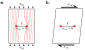
\includegraphics[scale=1]{../Figures_chap_article/crack_griffith.pdf}
\caption[Concentration des contraintes en pointe de fissure]{Représentation schématique de deux fractures. \textbf{a.}\,Fracture de longueur $\ell$ en mode d'ouverture. Une contrainte d'étirement $\sigma_{yy}$ homogène est appliquée au système. Les lignes rouges représentent les lignes de force dans le matériau. Une concentration des lignes de force indique une augmentation de la contrainte locale\,\cite{ohring_engineering_1995}. \textbf{b.}\,Fracture de longueur $\ell$ en mode de cisaillement dans le plan. Une contrainte de cisaillement $\sigma_{xy}$ homogène est appliquée au système. Les cercles rouges indiquent une concentration des contraintes.}
\label{fig:griffith_intro}
\end{figure}




Lorsqu'une contrainte $\sigma$ est appliquée aux bords d'un matériau élastique isotrope, elle est transmise à l'intérieur de celui-ci selon la loi de Hooke. Si le milieu est homogène, chaque volume infinitésimal du matériau supporte la même contrainte, mais si un défaut apparaît, il peut être le siège d'une concentration des contraintes, ce qui en fait un point de faiblesse du matériau. Une \textit{fracture}, ou \textit{crack}, ou encore \textit{rupture}, est un défaut du matériau consistant en une surface le long de laquelle les contraintes sont nulles.

Un exemple de fracture dans un matériau soumis à une contrainte d'extension est une déchirure dans une feuille mince que l'on étire (Fig.\,\ref{fig:griffith_intro}a). Lors de l'étirement de la feuille, les bords de la déchirure ne supportent aucune contrainte $\sigma_{yy}$. Sa pointe en revanche accumule de plus grandes contraintes que le reste du matériau, ce qui mène à terme à sa propagation, et à la déchirure complète de la feuille. C'est par l'existence de ce type de fractures que Griffith a répondu à la question initiale de son étude portant sur les fibres de verre. Les microfissures dans le verre, dues aux imperfections de fabrication, mènent à une accumulation de contraintes et à la rupture précoce de l'échantillon\,\cite{griffith_phenomena_1921}.












\subsubsection{Critère d'initiation de Griffith}


Si une fracture est présente dans un matériau au repos, elle ne se propage pas. Lorsque le matériau est chargé et la contrainte appliquée à l'interface est suffisante, la fracture peut s'étendre. Cette contrainte limite $\sigma_c$ dépend des propriétés du matériau, mais également de la longueur de la fracture. Afin de la déterminer il nous faut effectuer un bilan d'énergie. Deux énergies sont en jeu dans la propagation d'une fracture. La première est l'énergie potentielle élastique stockée par le matériau en raison des déformations. L'énergie potentielle élastique totale du matériau $E_{el}$ s'exprime grâce à la densité d'énergie potentielle locale $e_{el}$ par

\begin{equation}
E_{el} = \iiint e_{el}\,\mathrm{d}\mathcal{V}\qquad\text{avec}\qquad e_{el}=\frac{1}{2}\varepsilon\cdot\sigma
\end{equation}


Dans un matériau contenant une fracture, celle-ci créé une ligne de contraintes nulles, et relâche une partie de cette énergie par rapport au matériau sans défaut. L'énergie relâchée par unité de longueur du crack est notée $W$. Nous définissons $G=-\partial W/\partial\ell$ le \textit{taux de restitution d'énergie} (\textit{energy release rate}) correspondant à l'énergie libérée par la propagation de la fracture par unité de longueur. Il nous faut ensuite considérer l'énergie nécessaire à la création du défaut par unité de longueur, notée $U$. La fracture ne peut se propager que lorsque les variations de ces deux énergies linéiques avec la longueur du crack $\ell$ se compensent. Le critère de Griffith est alors que l'énergie libérée par le relâchement élastique compense l'énergie nécessaire à la création des surfaces libres, soit

\begin{equation}
\dfrac{\partial\:}{\partial\ell}\left(W-U\right)=0
\end{equation}

Dans son article fondateur Griffith considère le cas d'une plaque mince contenant une fissure de le longueur $\ell$ et soumise à une contrainte en ouverture $\sigma$ uniforme et constante, dans l'hypothèse de planéité des contraintes\,\cite{griffith_phenomena_1921}. Il montre alors que

\begin{equation}
W\propto \ell^2\sigma^2/E
\end{equation}

De plus l'énergie $U$ peut s'exprimer en fonction de la longueur de la fissure à l'aide de \textit{l'énergie de fracture} $\Gamma$, qui est une caractéristique du matériau, sous la forme

\begin{equation}
U = \Gamma \ell
\end{equation}

Ainsi le critère de Griffith devient

\begin{equation}
G=\Gamma
\end{equation}


Cette équation permet d'établir l'expression d'une contrainte limite $\sigma_c$ à partir de laquelle la fracture se propage\,\cite{griffith_phenomena_1921,freund_dynamic_1990}

\begin{equation}
\sigma_c\propto\sqrt{\frac{\Gamma E}{\ell}}
\end{equation}

Ainsi la contrainte $\sigma_c$ nécessaire pour déstabiliser une fracture est une grandeur décroissante de la longueur de celle-ci. La valeur exacte de cette contrainte dépend de la géométrie considérée. Dans le cas d'un système de taille infinie avec un chargement homogène en ouverture\,\cite{sun_fracture_2012}


\begin{equation}
\sigma_c=\sqrt{\frac{\Gamma E}{\pi\ell(1-\nu^2)}}
\end{equation}


Il est possible de considérer $\Gamma$ comme la valeur critique de $G$, notée également $G_c = \Gamma$. Conjointement la longueur de Griffith est définie comme la longueur critique $\ell_c\propto1/\sigma^{2}$ telle que $G=\Gamma$.


Ce critère nous permet de déterminer le point critique pour lequel la fracture s'initie, mais ne nous renseigne pas sur la forme que prennent les contraintes à son passage. Les contributions de G.\,R.\,Irwin et M.\,L.\,Williams (1957)\,\cite{irwin_analysis_1957,williams_stress_1957} ont éclairé ce point, et nous permettent de déterminer la forme du tenseur des contraintes au voisinage de la fracture, et en particulier à sa pointe.






\subsubsection{Facteur d'intensité des contraintes}
\begin{figure}[htb]
\centering

\includegraphics[scale=1]{../Figures_chap_intro/polaire.pdf}
\caption[Coordonnées polaires]{Définition des coordonnées polaires dans le cadre de la propagation d'une fracture. Le repère généralement utilisé pour décrire une fracture est solidaire de sa pointe, définissant $r$ comme la distance à celle-ci et $\theta$ l'angle par rapport à la direction de propagation.}
\label{fig:polaire}
\end{figure}


Lorsqu'un matériau contient une fissure, les tenseurs des contraintes et déformations en son sein sont altérés. En effet les coins de la fissure concentrent de fortes contraintes, tandis qu'elles sont nulles le long de la fissure. Dans le cadre de l'étude d'un solide idéalement élastique et linéaire il est possible de déterminer leur expression à proximité de la pointe de la fissure\,\cite{irwin_analysis_1957,williams_stress_1957,erdogan_fracture_2000,sun_fracture_2012}.


Nous repérons la position d'un point dans le matériau par ses coordonnées polaires $(r,\theta)$ par rapport à la pointe de la fissure (Fig.\,\ref{fig:polaire}). La résolution des équations de l'élasticité sous les hypothèses considérées donne l'expression générale du tenseur $\sigma_{ij}$ en un point $(r,\theta)$ sous la forme d'un développement en séries de Williams\,\cite{williams_stress_1957} comme suit, où les fonctions $g_{ij}^n$ sont des fonctions angulaires connues

\begin{equation}
\sigma_{ij}=\sum_{n=-1}^{+\infty} A_n\,r^{n+1/2}\,g^n_{ij}(\theta)
\end{equation}

Ce développement en puissances de $r$ ne prend que des valeurs demi-entières. Il commence en $n=-1$ pour satisfaire la convergence de l'énergie en pointe de fissure. Pour le montrer nous nous plaçons dans les coordonnées cylindriques, $\mathrm{d}\mathcal{V}(r)=r\mathrm{d\theta}\,\mathrm{d}r\,\mathrm{d}z$. Si nous considérons un des termes $\sigma = r^{\lambda}$ du développement, l'énergie élastique associée contenue en pointe de fissure dans un cercle de rayon $r$ est

\begin{equation}
\begin{aligned}
W(r)&=\frac{1}{2}\iiint\sigma\cdot\varepsilon\,\mathrm{d}\mathcal{V}(r)\propto \int_{0}^r \rho_r^{2\lambda+1}\,\mathrm{d}\rho_r
\end{aligned}
\end{equation}

Ainsi l'énergie contenue en pointe de fissure ne converge donc que si $\lambda > -1$.

À grande distance de la pointe de fissure, le tenseur des contraintes est régi par les termes tels que $n\geq0$. Cependant à proximité de la pointe, le terme en $n=-1$ diverge, et domine donc tous les autres. Par conséquent l'expression des contraintes en pointe de fissure peut être donnée par le développement limité suivant\,\cite{sun_fracture_2012}

\begin{equation}
\sigma_{ij} = \frac{K}{\sqrt{2\pi r}}f_{ij}(\theta)+\Theta\left(r^{1/2},r^{3/2},\dots\right)
\label{eq:joceline}
\end{equation}

Dans cette équation les $f_{ij}=g_{i,j}^{n=-1}$ sont des fonctions universelles dont l'expression est ·connue, et $K$ est nommé \textit{facteur d'intensité des contraintes}. Cette quantité, dont la valeur dépend de la géométrie du système et du chargement, fixe l'amplitude des contraintes subies par la pointe de fissure. Il est possible de reformuler le critère de Griffith en termes de facteur d'intensité des contraintes en définissant $K_c\sim\sqrt{\Gamma E}$ la \textit{ténacité} d'un matériau comme la valeur de $K$ lorsque $\sigma=\sigma_c$\,\cite{irwin_analysis_1957}. Cette valeur est une caractéristique du matériau. Pour le PMMA, $K_c\simeq\SI{1.1}{\mega\pascal\meter\tothe{1/2}}$\,\cite{ohring_engineering_1995}.

Le facteur d'intensité de contraintes $K$ prend la forme du produit de la contrainte à grande distance du crack et d'un facteur géométrique dépendant de la longueur du crack, il est donc possible de le calculer pour des géométries simples. Dans le cas général le calcul peut se décomposer par linéarité en un jeu de trois équations indépendantes selon des modes, comme présenté dans la section suivante.

Lorsque la contrainte atteint la limite de plasticité du matériau $\sigma_Y$ (Fig.\,\ref{fig:yield}), les déformations ne peuvent plus être considérées comme élastiques. La zone dans laquelle l'expression obtenue avec l'hypothèse d'élasticité n'est plus valable est nommée \textit{zone de régularisation des contraintes} (\textit{process zone}). Les considérations énergétiques associées aux phénomènes non-linéaires ayant lieu dans cette zone sont incorporées dans une définition plus générale de l'énergie de fracture.



\subsubsection{Modes de fracture}


\begin{figure}[htb]
\centering
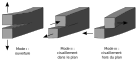
\includegraphics[scale=1]{../Figures_chap_intro/modes.pdf}
\caption[Modes de fracture]{Représentation des trois modes de fracture. Chaque mode évolue indépendamment des deux autres, ce qui permet de décomposer la solution générale des équations de la mécanique de la fracture linéaire élastique sur chacun d'eux.}
\label{fig:modes}
\end{figure}


Les fractures peuvent être décomposées en 3 modes selon le mode de chargement, c'est à dire la direction des contraintes appliquées relativement à leur direction de propagation\,\cite{freund_dynamic_1990,sun_fracture_2012} (Fig.\,\ref{fig:modes}). La fracture en ouverture est dite de \textit{mode\:\textsc{i}}, la contrainte nulle le long de la fracture est $\sigma_{yy}$. La contrainte nulle le long d'une fracture en cisaillement dans le plan, dite de \textit{mode\:\textsc{ii}}, est la contrainte cisaillante $\sigma_{xy}$. Le mode\:\textsc{iii} pour sa part correspond à un cisaillement hors du plan de propagation de la fracture. Il se caractérise par le fait que seuls les $\sigma_{zj}$ ne sont pas nuls partout. Dans le cadre de la fracture linéaire, en raison de la linéarité, ces trois modes peuvent être étudiés indépendamment, leurs contributions sont alors superposées pour décrire une fracture en mode mixte.

\newpage

Ainsi il est possible de décomposer $[\sigma]$ selon chacun de ces modes

\begin{equation}
[\sigma]=\sum_{\textsc{m}=\textsc{i,ii,iii}}[\sigma^\textsc{m}]
\end{equation}


Nous pouvons ensuite définir un facteur d'intensité des contraintes $K_\textsc{m}$ pour chaque mode puis décomposer l'Équation\,\ref{eq:joceline} comme

\begin{equation}
\sigma_{ij} = 
\sum_{\textsc{m}\in\{\textsc{i,ii,iii}\}}
\sigma_{ij}^\textsc{m}
\quad\text{avec}\quad
\sigma_{ij}^\textsc{m}=
\frac{K_\textsc{m}}{\sqrt{2\pi r}}f_{ij}^\textsc{m}(\theta)+\Theta\left(r^{1/2},r^{3/2},\dots\right)
\label{eq:sigmamodes}
\end{equation}




Les expressions des fonctions $f_{ij}^\textsc{m}$ sont alors les suivantes\,\cite{sun_fracture_2012}



\begin{equation}
\resizebox{150mm}{!}{
$
\begin{cases}
	f^\textsc{i}_{xx}&=\left(1-\sin\frac{\theta}{2}\,\sin\frac{3\theta}{2} \right)\cos\frac{\theta}{2}\\[.5em]
	f^\textsc{i}_{yy}&=\left(1+\sin\frac{\theta}{2}\,\sin\frac{3\theta}{2} \right)\cos\frac{\theta}{2}\\[.5em]
	f^\textsc{i}_{xy}&=\sin\frac{\theta}{2}\,\cos\frac{3\theta}{2}\,\cos\frac{\theta}{2}
\end{cases}
\quad
\begin{cases}
	f^\textsc{ii}_{xx}&=-\left(2+\cos\frac{\theta}{2}\,\cos\frac{3\theta}{2}\right)\sin\frac{\theta}{2}\\[.5em]
	f^\textsc{ii}_{yy}&=\cos\frac{\theta}{2}\,\cos\frac{3\theta}{2}\,\sin\frac{\theta}{2}\\[.5em]
	f^\textsc{ii}_{xy}&=\left(1-\sin\frac{\theta}{2}\,\sin\frac{3\theta}{2} \right)\cos\frac{\theta}{2}
\end{cases}
\quad
\begin{cases}
	f^\textsc{iii}_{zx}&=-\sin\frac{\theta}{2}\\[.5em]
	f^\textsc{iii}_{zy}&=\cos\frac{\theta}{2}\\
\end{cases}
$}
\end{equation}

L'expression de $f_{zz}^{\textsc{i},\textsc{ii}}$ dépend de l'hypothèse de planéité choisie
\begin{equation}
f_{zz}^{\textsc{i},\textsc{ii}}=
\begin{cases}
0&\quad\text{planéité des contraintes}\\
\nu(f_{xx}+f_{yy})&\quad\text{planéité des déformations}
\end{cases}
\end{equation}


L'expression des fonctions $f^\textsc{m}_{ij}$ en $\theta=0$ permet de donner une expression des $K_\textsc{m}$ permettant notamment leur mesure :

\begin{equation}
\begin{aligned}
K_\textsc{i}&=\lim_{\:r\rightarrow 0^+}\sqrt{2\pi r}\;\sigma_{yy}(r,\theta=0)\\
K_\textsc{ii}&=\lim_{\:r\rightarrow 0^+}\sqrt{2\pi r}\;\sigma_{xy}(r,\theta=0)\\
K_\textsc{iii}&=\lim_{\:r\rightarrow 0^+}\sqrt{2\pi r}\;\sigma_{zy}(r,\theta=0)
\end{aligned}
\end{equation}


La séparation de l'Équation\,\ref{eq:joceline} en modes indépendants permet également de définir des valeurs de $G$ par mode, notées $G_\textsc{m}$. L'expression complète de $G$ est alors donnée par
\begin{equation}
G=\frac{1-\nu^2}{E}\left(K_\textsc{i}^2+K_\textsc{ii}^2\right) + \frac{1+\nu}{E}K_\textsc{iii}^2
\end{equation}






\begin{figure}[p]
\centering
\begin{tabular}{lccc}
Matériau & $\Gamma\left(\mathrm{kJ.m}^{-2}\right)$ & $K_{I c}\left(\unit{\mega\pascal\meter\tothe{1/2}}\right)$ & $E(\mathrm{GPa})$ \\
\hline & & & \\
Acier allié & 107 & 150 & 210 \\
Aluminium allié & 20 & 37 & 69 \\
Acier & 12 & 50 & 210 \\
Caoutchouc & 13 & - & 0.001 \\
époxy & 2 & 2.2 & 2.4 \\
PMMA & 0.5 & 1.1 & 2.5 \\
Polystyrène & 0.4 & 1.1 & 3 \\
Bois & 0.12 & 0.5 & 2.1 \\
Verre & 0.007 & 0.7 & 70 \\
\hline
\end{tabular}
\caption[Caractéristiques de différents matériaux]{Caractéristiques de différents matériaux pour une fracture en mode\:\textsc{i} (extrait de\,\cite{ohring_engineering_1995}). Il est possible de montrer que $\Gamma\simeq K^2/E$.}
\label{tab:caracmater}
\end{figure}


\begin{figure}[p]
\centering
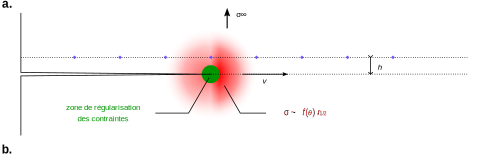
\includegraphics[scale=1]{../Figures_chap_intro/LEFM_plot_mesure.pdf}
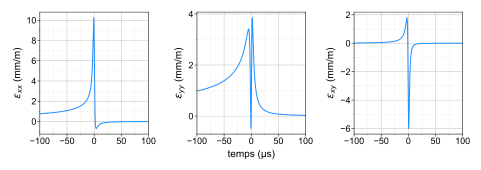
\includegraphics[scale=1]{../Figures_chap_intro/LEFM_plot.pdf}
\caption[Simulation d'une rupture dynamique en mode \textsc{i}]{\textbf{a.}\,Propagation et mesure d'une rupture en mode\:\textsc{i}. La rupture se propage le long de la ligne pointillée du bas à une vitesse $v$. Les capteurs de déformation mesurant $\varepsilon$ sont disposés le long de la ligne pointillée du haut, à une distance $h$ de la ligne de propagation de la rupture. Afin de mesurer le passage de la rupture et sa forme caractéristique, la distance $h$ doit être choisie supérieure au rayon de la zone de régularisation mais dans la zone où le terme en $\sigma\sim r^{-1/2}$ domine le développement en série de Williams. \textbf{b.}\,Évolution de $\varepsilon$ en fonction du temps au passage d'une fracture à $h=\SI{1}{\milli\meter}$ du point de mesure. L'oscillation en vaguelette observée est la signature de la fonction angulaire $\Sigma_{ij}^\textsc{m}$. La fracture se déplace à $v=\SI{500}{\meter\per\second}$, et l'énergie de fracture du matériau est $G=\SI{2}{\kilo\joule\per\meter\squared}$ (similaire à du PMMA).}
\label{fig:simulfrac}
\end{figure}








En résumé, nous avons vu qu'au sein d'un matériau, la pointe d'une rupture statique ou quasi-statique de longueur $\ell$ est le siège d'une concentration des contraintes. Le critère d'initiation de rupture de Griffith indique que lorsque le taux de restitution d'énergie $G$ est égal à l'énergie de fracture du matériau $\Gamma$ (Fig.\,\ref{tab:caracmater}), la fracture peut se propager, permettant la définition d'une contrainte limite $\sigma_c$ pour une rupture de longueur $\ell$. Cette contrainte s'exprime comme $\sigma_c\propto\sqrt{\Gamma E/\ell}$, le facteur de proportionnalité dépendant de la géométrie considérée. La contrainte en pointe de fissure s'exprime comme une série de Williams dont le terme dominant à proximité de la pointe de fissure est $\sigma\propto K/\sqrt{r}$, avec $K$ le facteur d'intensité des contraintes, qui lorsque la contrainte atteint $\sigma_c$ vaut $K = K_c$ la ténacité du matériau (Fig.\,\ref{tab:caracmater}). Nous avons enfin vu qu'il était possible de décrire tout crack comme la superposition de trois modes indépendants par linéarité. Cette séparation permet notamment de redéfinir les caractéristiques du matériau et critère d'initiation par mode.

Les trois modes ont leur propre critère d'initiation, et leur équation de propagation. L'évolution de la rupture est alors décrite par les lois de la fracture dynamique.


\subsection{Fracture dynamique}





Une fois déstabilisée, une rupture peut se propager dynamiquement dans le matériau. Si sa vitesse $v$ est telle que $v<c_r$ la vitesse des ondes de Rayleigh dans le matériau, la rupture est dite \textit{sub-Rayleigh}. Elle est alors décrite par la mécanique de la fracture linéaire élastique. Si cependant elle se déplace à $v>c_s$ la vitesse des ondes de cisaillement, elle est dite \textit{supershear}. Dans ce cas, la convergence du flux d'énergie élastique en point de fissure ne permet pas d'expliquer sa propagation, qui dépend d'un cadre physique différent\,\cite{dunham_supershear_2003}.

\subsubsection{Expression du tenseur des contraintes}


Dans le cas des ruptures sub-Rayleigh sous un chargement constant, l'expression de $\sigma_{ij}^\textsc{m}$ dépend de la vitesse, et en particulier des rapports $\alpha_s =\sqrt{ 1-(v/c_s)^2}$ et $\alpha_p =\sqrt{ 1-(v/c_p)^2}$ où $c_p$ et $c_s$ sont les vitesses des ondes de compression et de cisaillement dans le matériau. L'expression des facteurs d'intensité des contraintes est alors donnée par

\begin{equation}
K_\textsc{m}(v)=K_\textsc{m}^S\times k_\textsc{m}^d(v)
\end{equation}

Dans cette expression $K_\textsc{m}^S = K_\textsc{m}(v=0)$ correspond au facteur d'intensité des contraintes statique ou quasi-statique, et $k_\textsc{m}^d(v)$ est une fonction connue de la vitesse de propagation. Cette expression n'est valide que pour un système quasi-infini, pour lequel les ondes émises par la rupture n'ont pas eu le temps de se réfléchir sur un bord. Sous cette hypothèse il est possible de calculer $K_\textsc{m}(v)$.

Les fonction $f_{ij}^\textsc{m}(\theta)$ dans l'Équation\,\ref{eq:sigmamodes} sont également remplacées par des fonctions dynamiques $\Sigma_{ij}^\textsc{m}(\theta,v)$ connues, exhibant en modes \textsc{i} et \textsc{ii} une divergence lorsque $v\rightarrow c_r$, et lorsque $v\rightarrow c_s$ en mode \textsc{iii}. L'expression du tenseur des contraintes en pointe de fissure est alors donnée par\,\cite{sun_fracture_2012}


\begin{equation}
\sigma_{ij}^\textsc{m}=\frac{K_\textsc{m}^Sk^d_\textsc{m}(v)}{\sqrt{2\pi r}}\Sigma^\textsc{m}_{ij}(\theta,v)+\Theta(r^{1/2},r^{3/2},\dots)
\label{eq:sigmamodedyn}
\end{equation}

Lors du passage d'une rupture à proximité d'un capteur de déformation, la coordonnée $\theta$ repérant le point de mesure dans le référentiel de la pointe de fissure passe de $\theta\rightarrow\SI{0}{\degree}$ à $\theta\rightarrow\SI{180}{\degree}$. Ainsi la mesure balaie la fonction angulaire $\Sigma_{ij}^\textsc{m}$ et exhibe une variation caractéristique en vaguelette (Fig.\,\ref{fig:simulfrac}). La mesure de $\varepsilon$ au passage de la rupture permet de déterminer $\Gamma$ par un ajustement\,\cite{svetlizky_brittle_2019}.

\newpage


\subsubsection{Critère de propagation}

Le critère de propagation d'une rupture dynamique est identique au critère d'initiation d'une rupture statique, c'est à dire que le taux de restitution d'énergie $G$ doit être égal à l'énergie de fracture $\Gamma$, mais $G$ dépend de la vitesse de propagation. Il est possible d'exprimer $G$ sous la forme

\begin{equation}
G(v)\propto\frac{K^2}{E}\times A(v)\quad\text{et}\quad G(v) = \Gamma
\label{eq:propagfracdyn}
\end{equation}

La fonction $A(v)$, nommée facteur dynamique, prend en mode\:\textsc{i} et \textsc{ii} la forme

\begin{equation}
A(v)=\dfrac{\alpha_p(1-\alpha_s^2)}{4\alpha_p\alpha_s-(1+\alpha_p^2)^2}
\end{equation}

Ce facteur diverge lorsque $v\rightarrow c_r$ la vitesse des ondes de Rayleigh, correspondant à la première racine réelle du dénominateur de $A(v)$. Cette égalité indique que l'énergie nécessaire à la propagation d'une rupture sub-Rayleigh en mode\:\textsc{i} ou \textsc{ii} diverge lorsque la vitesse de propagation approche $c_r$, ce qui en fait la vitesse maximale de ce type de rupture. Pour une rupture en mode\:\textsc{iii} la vitesse limite est $c_s$.






\subsection{Fracture frictionnelle}
\label{sec:LEFMfric}



Pour décrire la mise en glissement d'une interface frictionnelle,
l'extension spatiale de celle-ci doit être considérée, contrairement à l'approche adoptée dans les modèles Rate-and-State, qui décrivent le mouvement du centre de masse du système
(Sec.\,\ref{sec:rateandstate}). En effet cette initiation du mouvement est due à un affaiblissement de l'interface par un front propagatif qui peut s'assimiler à un front de rupture. Il a été montré que ce front est une fracture en mode de cisaillement décrite par la mécanique de la fracture linéaire élastique\,\cite{svetlizky_brittle_2019}. Dans cette section nous présentons les spécificités théoriques de la fracture frictionnelle.


\subsubsection{Phénoménologie}

Une rupture fragile classique amorcée en un point de l'espace se propage dans le matériau alentour en raison de l'accumulation des contraintes en sa pointe, rompant le bloc le long de sa trajectoire. Dans le cas d'une rupture frictionnelle, l'interface est pressée et chargée à grande distance et accumule des contraintes cisaillantes. La rupture peut alors nucléer en un point de l'interface où un microcontact atteint sa résistance au cisaillement, se rompt et se met en glissement (Sec.\,\ref{sec:microfric}). Cette mise en glissement reporte les contraintes que le contact portait sur les aspérités avoisinantes, rompant de proche en proche ces microcontacts le long de l'interface. La rupture peut se propager ainsi tout le long de l'interface, jusqu'à avoir affaibli tous les contacts, permettant le glissement inertiel des blocs. Ces ruptures, comme les ruptures en mode de cisaillement classique, se propagent à des vitesses $v$ telles que $v<c_r$ la vitesse des ondes de Rayleigh dans le matériau, ou telles que $v>c_s$ la vitesse des ondes de cisaillement.

Le mouvement de glissement macroscopique des deux blocs est un mouvement inertiel, il ne commence qu'après que la rupture a traversé l'interface entière. Lorsque les blocs ont relâché une quantité suffisante des contraintes cisaillantes, le glissement s'arrête et les microcontacts se reforment (Sec.\,\ref{sec:evolutionmacro}). L'interface peut alors se recharger, et entrer par exemple dans un cycle de stick-slip, pour lequel chaque évènement de slip est initié par une rupture.

Nous présentons dans la section suivante que la propagation de ces ruptures est régie par la mécanique de la fracture.


\subsubsection{Description par la mécanique de la fracture}

La fracture frictionnelle est une fracture en mode\:\textsc{ii}, guidée par un plan faible formé par l'interface. Ce guidage est une composante essentielle de sa propagation, car dans un solide intact, une fracture initiée en mode\:\textsc{ii} est instable, et évolue spontanément vers le mode\:\textsc{i}. Le long de l'interface frictionnelle, l'énergie de fracture associée à l'affaiblissement des microcontacts $\Gamma_\textsc{fric}$ est beaucoup plus faible que celle associée à une fracture du matériau intact $\Gamma_\textsc{bulk}$. Guidée par l'interface, la rupture peut être repérée par la coordonnée $x(t)$ de son front, et il n'est pas exclu que $\Gamma_\textsc{fric}$ dépende de $x$. Ainsi à partir de l'Équation\,\ref{eq:propagfracdyn} nous pouvons écrire

\begin{equation}
\Gamma_\textsc{bulk} \gg \Gamma_\textsc{fric}
\quad\text{et}\quad
G_\textsc{ii}(v) = \Gamma_\textsc{fric}(x)
\end{equation}


Une différence majeure entre une fracture classique et une rupture frictionnelle est que la rupture frictionnelle n'est pas une ligne de contraintes nulles. En effet, là où après le passage d'une rupture classique le matériau est endommagé de manière irréversible, la rupture frictionnelle affaiblit des microcontacts et leur permet de se mettre en mouvement. Les microcontacts supportent toujours après le passage de la rupture une contrainte cisaillante résiduelle $\sigma_{xy} =\sigma_r$ (Sec.\,\ref{sec:microfric}). De plus pour une rupture en mode de cisaillement les contraintes initiales le long de la ligne de propagation de la rupture sont

\begin{equation}
\big[\sigma^\textsc{ii}\big] (\theta = 0,\,r\rightarrow+\infty) = \begin{bmatrix}
0 & \sigma_{xy}^0\\
\sigma_{xy}^0 & 0
\end{bmatrix}
\label{eq:initnormal}
\end{equation}

Ainsi afin de ramener le tenseur des contraintes $[\sigma^\textsc{fric}]$ d'une rupture frictionnelle à celui d'une fracture en mode de cisaillement, la linéarité des équations présentées permet de prendre en compte les conditions initiales par superposition

\begin{equation}
\big[\sigma^\textsc{ii}\big] = 
\big[\sigma^\textsc{fric}\big] -
\begin{bmatrix}
\sigma_{xx}^0 & \sigma_r\\
\sigma_r      & \sigma_{yy}^0
\end{bmatrix}
\label{eq:pmpi}
\end{equation}


Il a de plus été montré que les contraintes divergent en pointe de fissure selon les équations de la mécanique de la fracture linéaire élastique\,\cite{svetlizky_classical_2014}. Elle est dont décrite par l'Équation\,\ref{eq:sigmamodedyn} avec $\textsc{m}=\textsc{ii}$ seulement, c'est à dire





\begin{equation}
\sigma_{ij}^\textsc{fric}
=
\frac
	{K_{\textsc{ii}}(v)}
	{\sqrt{2\pi r}}
\times
	\Sigma_{ij}^{\textsc{ii}}
(\theta,v)
+
\begin{bmatrix}
	\sigma_{xx}^0 & \sigma_r\\
	\sigma_r      & \sigma_{yy}^0
\end{bmatrix}
\label{eq:fracdynfric}
\end{equation}

Dans cette équation $K_\textsc{ii}$ est le facteur d'intensité des contraintes lié à l'énergie de fracture de l'interface frictionnelle $\Gamma = \Gamma_\textsc{fric}$. Cette énergie correspond à l'énergie nécessaire pour affaiblir les microcontacts à l'interface, elle est donc directement liée à l'aire réelle de contact $A_r$, elle-même proportionnelle à $\sigma_{yy}$\,\cite{svetlizky_brittle_2019}. Ainsi

\begin{equation}
\Gamma(x)\propto\sigma_{yy}(x)
\label{eq:homospa}
\end{equation}

Cette rupture frictionnelle a été largement étudiée dans le cas des interfaces solide-solide homogènes, comme présenté dans le Chapitre\:\ref{chap:etatdelart}.

Nous avons au cours de cette section montré que le mouvement de glissement rapide d'une interface frictionnelle est initié par la propagation d'une fracture le long de l'interface. Cette fracture est décrite de manière quantitative par la mécanique de la fracture linéaire élastique. Une question est de savoir si cette description est généralisable à des interfaces complexes comme celles étudiées en mécanique des failles, bien que leur comportement en découle. L'étude de celles-ci est présentée dans la section suivante.

\newpage








\section{Mécanique des failles}
\label{sec:failles}






La mécanique des failles est le domaine de la géophysique étudiant les mécanismes de déformations des roches et des failles sismiques, au travers d'échelles de temps et d'espace très diverses. Dans le cadre de notre étude d'une faille en laboratoire nous cherchons à caractériser des mouvements de glissement rapide à l'interface, qui s'apparentent à des séismes, un des objets d'étude de la mécanique des failles. Nous présentons dans cette section les principes de base de l'étude des mouvements lithosphériques, de la tectonique des plaques, et de la mesure et la caractérisation des séismes.


\begin{figure}[hbt]
\centering

\includegraphics[scale=1]{../Figures_chap_article/failles.pdf}
\caption[Types de failles]{Les trois grands types de failles. La faille normale (\textbf{a}) apparaît dans les systèmes en extension. La faille inverse (\textbf{b}) apparaît dans les systèmes en compression comme les zones de subduction. La faille transformante (\textbf{c}) apparaît dans les zones de coulissement entre des plaques tectoniques.}
\label{fig:typesdefailles2}
\end{figure}

\subsection{Qu'est-ce qu'une faille ?}

En géologie, une \textit{faille} est un plan ou une zone de rupture entre deux blocs rocheux qui sont en déplacement relatif. Les failles peuvent être de grandes dimensions, comme les failles tectoniques, ou millimétriques. Ces failles peuvent former des plans de ruptures très nets et très actifs, comme la faille de San Andreas à l'ouest des États-Unis\,\cite{scholz_evidence_2000}, ou de grandes zones de rupture contenant de multiples failles individuellement peu actives comme le rift est-africain\,\cite{chorowicz_east_2005}.




\subsubsection{Origine des failles}


La croûte terrestre, ou \textit{lithosphère}, est composée de plaques en mouvement relatif. Ces plaques, dites \textit{plaques tectoniques}, d'une épaisseur d'environ \SI{100}{\kilo\meter}\,\cite{pollack_regional_1977}, sont composées de roches basaltiques et granitiques solides et rigides, et reposent sur l'\textit{asthénosphère}, ou manteau terrestre, composé pour sa part de péridotites dans un état solide, mais ductile (Fig.\,\ref{fig:tecto}a). Le manteau, d'une épaisseur de l'ordre de \SI{3000}{\kilo\meter}, a une viscosité de l'ordre de $10^{18}$ à $10^{22}$\,Pa.s  contre $10^{25}$ pour la lithosphère\,\cite{cathles_viscosity_2015}, et peut ainsi, sous l'influence des gradients de température au sein de la Terre, adopter un mouvement de convection (Fig.\,\ref{fig:tecto}b). Ces mouvements forment des rouleaux, qui entraînent avec eux les plaques tectoniques à des vitesses allant jusqu'à \SI{10}{\centi\meter} par an.

De nombreux phénomènes géologiques ont lieu à l'interface entre les plaques tectoniques. Les zones d’accrétion, situées à l'interface entre deux plaques en éloignement, sont le siège d'un volcanisme à l'origine par exemple de la dorsale Atlantique qui émerge en Islande. Dans les zones de collision entre deux plaques, les mouvements tectoniques sont responsables de la subduction de la lithosphère océanique, engendrant du volcanisme d'arc, partiellement à l'origine de la lithosphère continentale\,\cite{stern_subduction_2002,Hawkesworth_generation_2010}. Des mouvements de coulissement entre les plaques tectoniques peuvent également se produire, comme c'est le cas le long de la faille de San Andreas\,\cite{anderson_san_1971, okubo_fractal_1987,zoback_new_1987, powell_evolution_1992, linde_slow_1996, tan_connecting_2020}. Les failles ont une morphologie sculptée par le temps et les contraintes qu'elles subissent.

\begin{figure}[hbt]
\centering
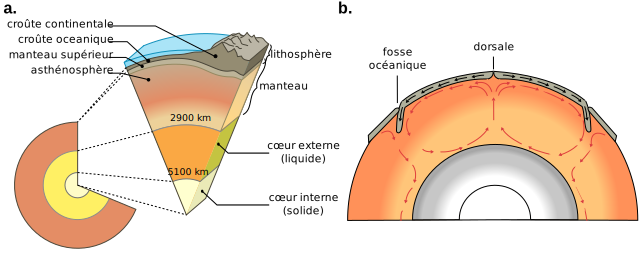
\includegraphics[scale=1]{../Figures_chap_intro/coupeterre.pdf}
\caption[Structure interne de la Terre]{Schéma de la structure interne de la Terre et du mécanisme par lequel les mouvements de convection du manteau sont à l'origine de la tectonique des plaques.}
\label{fig:tecto}
\end{figure}


\subsubsection{Anatomie d'une faille}



Une faille est un système géophysique complexe, centré sur un plan de faille, et composé de multiples couches de roches structurellement et chimiquement différentes. Lorsque deux blocs de roches en contact sont soumis à un déplacement relatif, ils subissent des contraintes et déformations menant à la fragilisation et à l'usure des roches. Il est ainsi possible d'observer de part et d'autre du plan de faille une succession de couches géologiques aux propriétés variées.

À grande distance du plan de faille, la roche mère forme un bloc solide, accumulant de l'énergie élastique au travers des déformations qu'elle subit. En s'approchant de la faille et en entrant dans la zone d'endommagement, celle-ci devient une \textit{cataclastite}, une roche de faille fracturée, broyée et stratifiée par le déplacement relatif des deux blocs en contact (Fig.\,\ref{fig:faillereelle}). Au centre de la zone de faille se trouve la zone cœur, composée de brèche de faille et de gouge, une roche granulaire non cohésive\,\cite{woodcock_classification_2008}. Au delà des différences de granulométrie, la différence de porosité entre ces couches introduit également des différences chimiques et métamorphiques. Enfin les failles sismiques ont une extension spatiale en profondeur, des séismes pouvant se produire jusqu'à 600 kilomètres sous la surface\,\cite{frohlich_nature_1989}. Chaque système de faille a sa morphologie propre.


\begin{figure}[h!]
\centering
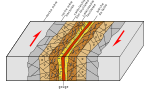
\includegraphics[scale=1]{../Figures_chap_article/realfault.pdf}
\caption[Anatomie d'une faille]{Anatomie schématique d'une faille sismique réelle. La faille est composée de multiples couches de roches, plus ou moins cohésives et fracturées. Les couches de brèche et de gouge sont des milieux granulaires au cœur de la faille (adapté de\,\cite{treffeisen_fault_2021}).}
\label{fig:faillereelle}
\end{figure}



\subsection{Étude des séismes}


Lorsque deux plaques tectoniques sont en contact, elles sont soumises à des forces de frottement solide. Les zones la plupart du temps bloquées en surface sont toujours soumises aux contraintes appliquées par les déplacements de l'asthénosphère, et accumulent de l'énergie élastique au travers de leurs déformations. Lorsqu'elles se débloquent, un évènement de glissement rapide a lieu. Cet évènement, relâchant l'énergie élastique accumulée, dure généralement au plus quelques secondes, et émet des ondes de déformations qui se propagent dans les roches alentour, parfois jusqu'à la surface. C'est ce mécanisme que l'on nomme \textit{séisme}.

%Les roches en contacts sont plus ou moins visqueuses selon les conditions de température et de pression dans lesquelles elles évoluent\,\cite{mccaffrey_slow_2008}, 



\subsubsection{Le stick-slip comme description du cycle sismique}

Les séismes sont la manifestation d'un mouvement de stick-slip. Cette observation, publiée en 1966 par W.\,F.\,Brace et J.\,D.\,Byerlee\,\cite{brace_stick-slip_1966}, s'appuyant alors sur les études menées en laboratoire sur des roches naturelles\,\cite{jaeger_frictional_1959,uffen_stress_1963,griggs_observations_1960}, est un fondement de l'étude moderne de la sismicité, remplaçant la théorie du rebond élastique de Reid\,\cite{reid_mechanics_1910}. Le mouvement de stick-slip est en effet caractéristique des dynamiques régies par les frottements solides (Sec.\,\ref{sec:ss1}).

Dans les mouvements géologiques ce mouvement de stick-slip ne se caractérise cependant pas par sa régularité, puisqu'il est très difficile de prédire les séismes\,\cite{rikitake_earthquake_1968, mogi_earthquake_1985, geller_earthquake_1997, kanamori_earthquake_2003}. La prédiction et prévention de ceux-ci est pourtant un enjeu majeur, et la compréhension des mécanismes microscopiques sous-jacents au frottement solide en est une clé. L'étude de ces mécanismes a mené à de nombreux modèles empiriques (Sec.\,\ref{sec:rateandstate}) appuyés par des observations de terrain permettant de décrire le comportement des failles et de rendre compte de ce phénomène de stick-slip à l'échelle des temps géologique.


\subsubsection{Magnitude et moment sismique}

Un séisme est la manifestation d'un glissement le long d'une interface frictionnelle. Il s'accompagne d'une dissipation d'énergie (Éq.\,\ref{eq:dissip}) et de l'émission et la propagation d'ondes dans les roches. La mesure de ces phénomènes permet de définir des grandeurs utiles à la caractérisation, au catalogage et à l'étude statistique des séismes. Nous définissons ici plusieurs de ces observables.


\myparagraph{Le déplacement moyen}

\begin{figure}[htb]
\centering
\includegraphics[width=.8\textwidth]{../Figures_chap_intro/fence.jpg}
\caption[Observation directe du glissement dû à un séisme]{Photographie des effets du tremblement de terre de 1906 à San Francisco, causé par la rupture d'une portion de la faille de San Andreas. La faille a glissé d'environ \SI{2.5}{\meter} le long d'un plan de fissure particulièrement bien défini\,\cite{reid_mechanics_1910}.}
\label{fig:fence}
\end{figure}

Le déplacement moyen est la moyenne de la distance glissée le long de la faille ou portion de faille rompue lors d'un séisme (Fig.\,\ref{fig:fence}). Son évaluation peut être effectuée par mesure directe des glissements sur le terrain, cependant dès lors que le mouvement est faible, ou que la zone de faille est étendue, elle perd en précision. Des techniques d'imagerie satellite ou de mesure par balises GPS permettent de raffiner ces mesures à une précision de l'ordre du centimètre, et de déterminer le champ des déformations dans toute la lithosphère\,\cite{michel_measuring_1999,segall_gps_1997,pagani_quantification_2021}. La mesure des déplacements en surface ne suffit cependant pas à caractériser un séisme, puisque certains mouvements profonds ne s'accompagnent pas d'un glissement en surface. Pour les caractériser des grandeurs liées à l'énergie qu'ils relâchent sont utilisées.


\myparagraph{Les magnitudes}

La \textit{magnitude} d'un séisme est une grandeur sans unité évaluant l'énergie libérée par ce séisme sur une échelle logarithmique. Sa définition a évolué au cours du temps, en fonction de la grandeur mécanique utilisée pour la mesurer. Historiquement la première définition est celle de Richter en 1935 de la magnitude locale $M_L$\,\cite{richter_instrumental_1935}. Elle est basée sur les mesures des ondes sismiques par des sismographes, appareils combinant des accéléromètres et vélocimètres, et est définie comme

\begin{equation}
M_L=\log(D)-\log(D_0)+c\times\log(\Delta)
\end{equation}

Dans cette équation, $D$ désigne l'amplitude maximale mesurée sur le sismogramme utilisé pour la mesure, $\Delta$ la distance à l'épicentre, $c$ une constante d'étalonnage, et $D_0$ une amplitude de référence déterminant ce que l'on considère comme la valeur de $D$ pour un séisme de magnitude $M_L=0$ perçu à \SI{100}{\kilo\meter}. Cette définition est aujourd'hui limitée à des études locales, car elle dépend de paramètres empiriques locaux, étalonnés par zone de faille. Cette limitation à mené à la définition des \textit{magnitudes d'ondes} basées chacune sur la mesure d'un type d'onde spécifique. Les deux magnitudes d'ondes sont celle des ondes de surface $M_S$ et celle des ondes de volume (\textit{body waves}) $m_b$ toutes deux introduites par Gutenberg et Richter en 1936 et 1956\,\cite{gutenberg_magnitude_1936,gutenberg_earthquake_1956}. Toujours en usage aujourd'hui, elles demeurent empiriques et basées sur des étalonnages, et subissent un phénomène de saturation lorsque $M_S$ ou $m_b>9$\,\cite{kanamori_energy_1977, howell_saturation_1981}.

La magnitude la plus couramment utilisée aujourd'hui est la \textit{magnitude de moment} $M_w$ introduite par Hanks et Kanamori en 1979\,\cite{hanks_moment_1979}, liée directement à l'énergie libérée par le séisme et au moment sismique. Elle est particulièrement utilisée pour les séismes de grande magnitude ($M>4$), tandis que les magnitudes d'ondes sont privilégiées pour les faibles magnitudes.

\myparagraph{Le moment sismique}

le \textit{moment sismique} $M_0$ est une mesure de l'énergie libérée par un séisme par l'évaluation du travail des forces responsables du glissement. À longue distance un séisme peut en effet être vu comme le résultat de l'application d'un double couple de forces\,\cite{kagan_3-D_1991} résultant en une déformation élastique des roches. Le moment s'exprime alors comme

\begin{equation}
M_0=\frac{E}{2(1+\nu)}\times A\times d
\end{equation}

Dans cette équation $G_s=E/2(1+\nu)$ est le module de cisaillement, $A$ est la surface macroscopique du plan de fracture rompue durant l'évènement, et $d$ est le déplacement moyen à l'interface. La magnitude de moment est alors définie comme

\begin{equation}
M_w=\frac{2}{3}\log_{10}(M_0)-6.07
\label{eq:magnitude}
\end{equation}

Une augmentation d'un point de magnitude correspond à une multiplication par 30 du moment sismique. La magnitude est ainsi définie sur une échelle à valeurs dans $\mathbb{R}$ nommée \textit{échelle de Richter}\,\cite{kanamori_quantification_1978}. L'échelle est théoriquement illimitée, cependant le séisme le plus fort enregistré est le séisme de 1960 à Valdivia au Chili, avec une magnitude $M_w=9.5$\,\cite{ruiz_historical_2018}. Les tremblements de terre d'une telle magnitude n'ont lieu qu'une à trois fois par siècle, et relâchent une quantité suffisante d'énergie pour altérer l'axe de rotation de la Terre et changer la longueur du jour de quelques microsecondes\,\cite{chao_changes_1987}. Bien que l'échelle n'ait théoriquement pas non plus de minimum, les séismes de magnitude inférieure à 1 sont très difficilement détectables et se produisent en continu sur Terre. Ils peuvent même être dus aux activités humaines, un séisme de magnitude 0 relâchant une quantité d'énergie équivalente à celle libérée par la
chute d'un objet d'une tonne d'une hauteur de \SI{5}{\meter}.
%\href{https://youtu.be/e3uk7jU3RHo}{\textcolor{black}{chute d'un objet d'une tonne d'une hauteur de \SI{5}{\meter}}.}

Dans le but de décrire et prévenir les risques sismiques, le moment sismique et la magnitude font l'objet d'études statistiques et de modèle empiriques, comme la loi de Gutenberg-Richter.


\subsubsection{Loi de Gutenberg Richter}

\label{sec:gutricht}

\begin{figure}[htb]
\centering
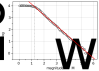
\includegraphics[scale=1]{../Figures_chap_intro/grlaw.pdf}
\caption[Loi de Gutenberg-Richter]{Distribution fréquence-magnitude cumulée des évènements sismiques dans la région de Abruzzi en Italie, entre avril 2007 et avril 2010 (adapté de\,\cite{de_santis_gutenberg-richter_2011}). Un séisme de magnitude $M_w=6.3$ a eu lieu dans la zone surveillée le 6 avril 2009. Un ajustement de la portion linéaire de la distribution (ligne rouge) permet une estimation globale des paramètres de la loi de Gutenberg-Richter ($b=0.89\pm0.03$). La ligne verticale en pointillés représente une estimation de la magnitude minimale à partir de laquelle les sismographes perdent leur sensibilité.}
\label{fig:grlaw}
\end{figure}

La loi de Gutenberg-Richter est une loi empirique décrivant la distribution de magnitude des séismes dans un réseau de failles donné\,\cite{gutenberg_frequency_1944}. Cette loi exprime un lien entre la magnitude $M$ et le nombre total de séismes d'une magnitude inférieure à $M$ ou \textit{distribution fréquence-magnitude cumulée} noté $N_{>M}$. La loi de Gutenberg-Richter prédit qu'il existe des constantes $a$ et $b$ telles que
\begin{equation}
\log_{10}N_{>M}=a-bM
\label{eq:grlaw}
\end{equation}


La loi de Gutenberg-Richter, bien qu'empirique, dispose d'un bon accord avec les données des relevés sismiques (Fig.\,\ref{fig:grlaw}). Les paramètres de la loi sont cependant variables d'un système de failles à un autre, et sont mesurés par région sismique. L'accord aux données de terrain n'est valable qu'à partir d'une magnitude minimale $M^-$ car les évènements de magnitude inférieure ne sont pas détectés par les sismographes.

D'autres évènements de glissement peuvent échapper aux sismographes, comme les séismes lents (\textit{slow earthquakes})\,\cite{beroza_searching_1990}.
\vspace{1cm}
\pagebreak

\subsection{Mouvement asismique}

Le mouvement asismique est défini comme le glissement d'une portion de faille ne durant non pas quelques secondes comme un séisme mais des temps plus grands, allant de l'ordre de la minute à plusieurs années. Certaines failles sont même dites \textit{découplées}, c'est à dire en glissement permanent. Ces glissements ont été mesurés comme ayant des magnitudes allant jusqu'à $M_w=7$\,\cite{liu_recurrent_2015}. Le rôle de ce glissement lent dans le cycle sismique, et en particulier son influence dans le déclenchement de séismes de grande magnitude, ou au contraire dans le relâchement des contraintes, est un sujet de recherche actif et reste encore méconnu\,\cite{harris_large_2017, radiguet_triggering_2016,burgmann_geophysics_2018, leeman_frictional_2018,tan_connecting_2020}.


La compréhension des mécanismes entraînant le glissement lent de portions de failles ainsi que l'influence de ce glissement partiel d'une faille ou d'un système de failles sur ses portions bloquées sont deux motivations de notre étude. En particulier les expériences présentées dans le Chapitre\,\ref{sec:chaparticle} exposent un mécanisme par lequel ce glissement lent d'une portion d'une interface frictionnelle peut mener à une déstabilisation précoce, mais donc de magnitude moindre, du reste de l'interface.













\section{Conclusion}

Nous avons abordé au cours de ce chapitre des notions importantes de trois domaines de la physique dont le sujet de notre étude est à l'interface. Notre étude vise en effet à explorer le comportement d'interfaces frictionnelles en présence d'une hétérogénéité de contrainte ou de composition. Ces interfaces peuvent tout d'abord être décrites par la mécanique des frottements à travers de modèles empiriques et microscopiques. La mécanique de la fracture linéaire élastique nous permet pour sa part de détailler les mécanismes microscopiques à l'œuvre à l'interface lors de la mise en glissement de 2 solides frottants. La mécanique des failles enfin met en perspective notre étude et les résultats présentés dans un cadre plus large et appliqué.

%Les outils, concepts et références bibliographiques que nous avons introduit ici nous permettent d'aborder les problématiques soulevées par notre étude sous plusieurs angles complémentaires. Les résultats principaux que nous avons présentés sont tout d'abord, pour la Section\,\ref{sec:frot}, l'émergence du mouvement de stick-slip à partir des lois de frottement. Ce mouvement est dû à la différence entre le coefficient de frottement statique $\mu_s$ et le coefficient de frottement dynamique $\mu_d$. Il apparaît dans l'ensemble des expériences que nous avons mené. Ensuite, dans la Section\,\ref{sec:LEFM}, nous avons présenté le comportement d'une fracture au sein d'un matériau, en particulier sa déstabilisation à partir d'une contrainte limite selon le critère de Griffith. Nous avons également détaillé l'initiation d'un mouvement de glissement par la propagation d'une fracture en mode de cisaillement à l'interface. Enfin dans la Section\,\ref{sec:failles} nous avons présenté les séismes comme une manifestation d'un mouvement de stick-slip, introduits des concepts de géophysique tels que la magnitude. Nous avons aussi présenté brièvement les séismes lents, glissement de portions de failles sur des temps longs entre les évènements sismiques.











